\documentclass[12pt]{article}
% math symbols
\usepackage{amssymb,amsmath}
% for different compilers
\usepackage{ifpdf}
% geometry of page
\usepackage[margin=2cm]{geometry}
% float pictures
\usepackage{wrapfig}

% if pdflatex, then
\ifpdf
 \usepackage[english,russian]{babel}
 \usepackage[utf8]{inputenc}
 \usepackage[unicode]{hyperref}
 \usepackage[pdftex]{graphicx}
 \usepackage{cmlgc}
% if xelatex, then
\else
% math fonts
 \usepackage{fouriernc}
% xelatex specific packages
 \usepackage[xetex]{hyperref}
 \usepackage{xunicode}	% some extra unicode support
 \usepackage{xltxtra}	% \XeLaTeX macro
 \defaultfontfeatures{Mapping=tex-text}
 \usepackage{polyglossia}	% instead of babel in xelatex
 \setdefaultlanguage{russian}
% fonts
 \setromanfont{Charis SIL}
 \setsansfont{TextBookC} 
 \setmonofont{Consolas}
\fi

% several pictures in one figure
\usepackage{subfig}
% calc in TeX expressions
\usepackage{calc}
% nice pictures and plots
\usepackage{pgfplots,tikz,circuitikz}
% different libraries for pictures
\usetikzlibrary{%
  arrows,%
  calc,%
  patterns,%
  decorations.pathreplacing,%
  decorations.pathmorphing,%
  decorations.markings%
}
\tikzset{>=latex}

% colors of the hyperlinks
\hypersetup{colorlinks,%
  citecolor=blue,%
  urlcolor=blue,%
  linkcolor=red
}

\tolerance=1000
\emergencystretch=0.74cm

\newcommand{\nn}{\nonumber}
\newcommand{\pt}{\partial}
\newcommand{\unit}[1]{\text{ #1}}
\newcommand{\eps}{\epsilon}
\newcommand{\vareps}{\varepsilon}
\newcommand{\const}{\mathrm{const}}
\newcommand{\com}[1]{{\Large{\texttt{{\color{red}(#1)}}}}}

% счётчик задач
\newcounter{notask}
\setcounter{notask}{1}

% условие без картинки
\newcommand{\task}[1]{
	\hrule
	\hbox to \textwidth {%
    	\vrule
	    \parbox[t]{0.04\textwidth}{\smallskip \centering \arabic{notask}}%
    	\vrule%
	    \hfill%
    	\parbox[t]{0.93\textwidth}{\smallskip #1 \smallskip}\hfill%
	    \vrule
	}
	\hrule
    \addtocounter{notask}{1}
    \pagebreak[2]
}

\newlength{\h}
\newsavebox{\taskbox}
\newlength{\x}
\newsavebox{\pictbox}

% условие с картинкой (картинка выравнивается по центру)
\newcommand{\taskpic}[2]{
	\savebox{\taskbox}{\parbox[t]{0.93\textwidth-4.3cm}{\smallskip #1 \smallskip}}
	\savebox{\pictbox}{\parbox[t]{4cm}{\smallskip \centering
    	\vspace{0pt} #2 \smallskip}}
	\h=\ht\taskbox
	\advance\h\dp\taskbox
	\x=\ht\pictbox
	\advance\x\dp\pictbox
	\hrule
	\hbox to \textwidth {%
		\vrule\parbox[t][\maxof{\h}{\x}][t]{0.04\textwidth}{ \smallskip
    		\centering \arabic{notask} }\vrule%
	    \hfill\parbox[t][\maxof{\h}{\x}][t]{0.93\textwidth-4.3cm}{\smallskip #1
    	    \smallskip}\hfill\vrule%
	    \hfill\parbox[t][\maxof{\h}{\x}][c]{4cm}{\hfil #2 \hfil}\hfill\vrule
	}
	\hrule
	\addtocounter{notask}{1}
	\pagebreak[2]
}

\tikzset{>=latex, interface/.style = {postaction = {draw, decorate,
	    decoration = {border, angle = 45, amplitude = 0.2cm, segment length=1.4323mm}}},%
		spring/.style={decorate,decoration={snake,amplitude=1mm,
        segment length=2mm},thick}}
      
\pagestyle{empty}

\begin{document}

\thispagestyle{empty}
\parindent=5mm
\righthyphenmin=2
\begin{center}

\phantom{Бухалкин апанас}

\vfill
\LARGE{\textsc{XVIII Летняя Физическая Школа}}\\
\Large{\textsc{17 июля -- 6 августа 2012}}\\[1cm]
\Large{\textit{Сборник материалов}}\\[2cm]
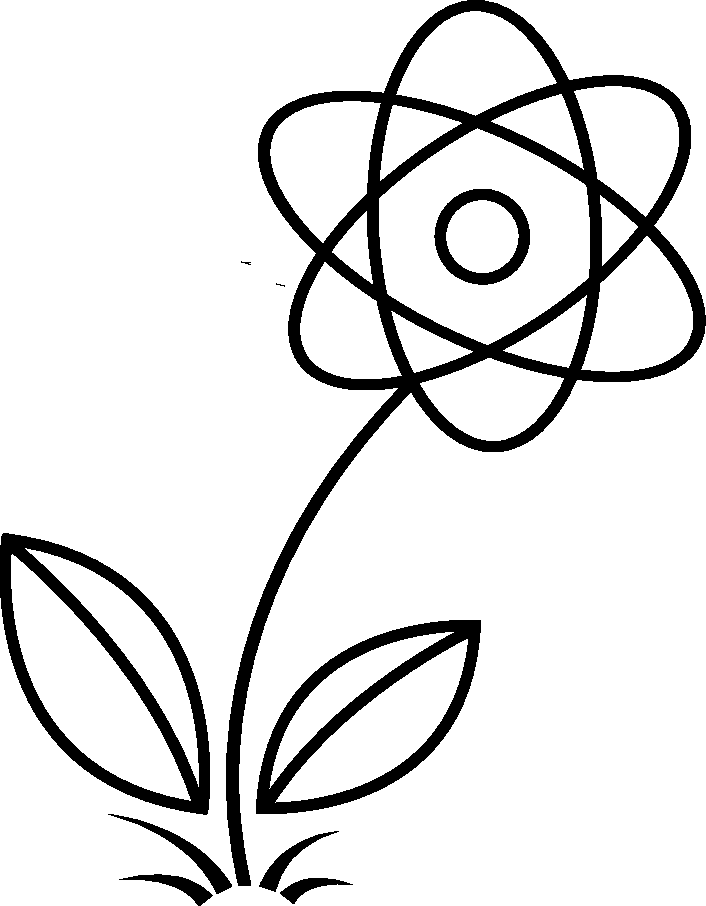
\includegraphics[width=7cm]{./logo2012.pdf}
\vfill

\small{\textsc{Санкт-Петербург}\\
\textsc{2012}}
\end{center}

\clearpage

\section{Участники ЛФШ. }
\label{sec:participants}

В работе Летней Физической Школы приняли участие 106 школьников 7--11
классов и 16 преподавателей. В школу принимались победители городской
олимпиады по физике, завоевавшие дипломы, либо успешно написавшие
вступительную работу школьники, либо школьники, получившие
рекомендацию руководителя параллели в предыдущей ЛФШ.

\begin{table}[ht]
  \begin{minipage}[t]{0.48\linewidth}\centering
    \begin{center}
      \textit{8 класс}
    \end{center}
    \begin{tabular}[h]{|c|c|c|c|}
      \hline
      \textbf{№} & \textbf{Фамилия, имя} & \textbf{Шк.} & \textbf{Д/б}\\
      \hline
      1 & Антонюк Валерий & 344 & Д2\\ \hline
      2 & Арутюнян Дмитрий & 265 & 45 \\ \hline
      3 & Беличенко Дмитрий & 183 & Д3 \\ \hline
      4 & Беляков Леонид & 610 & 42 \\ \hline
      5 & Богданова Полина & 97 & ПО \\ \hline
      6 & Богомолов Михаил & 610 & Д2 \\ \hline
      7 & Болотовский Владислав & 554 & Д3 \\ \hline
      8 & Дементьева Маргарита & 239 & 55 \\ \hline
      9 & Дроздов Дмитрий & 457 & Д2 \\ \hline
      10 & Евдокимов Тимур & 526 & 41 \\ \hline
      11 & Елфимова Олеся & 98 & Д3 \\ \hline
      12 & Жмаев Платон & 427 & 49 \\ \hline
      13 & Жмудь Богдан & 209 & Д2 \\ \hline
      14 & Захаров Алексей & 366 & Д2 \\ \hline
      15 & Калашников Георгий & 410 & Д3 \\ \hline
      16 & Коган Анна & 610 & 65 \\ \hline
      17 & Люлина Елена & 111 & 56 \\ \hline
      18 & Марченко Максим & 239 & Д3 \\ \hline
      19 & Нагавкина София & 622 & Д3 \\ \hline
      20 & Осколков Денис & 144 & 42 \\ \hline
      21 & Репетун Лада & 278 & Д3 \\ \hline
      22 & Родионов Иван & 328 & Д2 \\ \hline
      23 & Румянцева Ольга & 534 & Д2 \\ \hline
      24 & Сахно Денис & 239 & 32 \\ \hline
      25 & Свирин Евгений & 582 & 53 \\ \hline
      26 & Семченко Дмитрий & 610 & ПО \\ \hline
      27 & Смирных Дмитрий & 239 & 50 \\ \hline
      28 & Терехов Александр & 406 & ПО \\ \hline
      29 & Усачёва Мария & 295 & Д3 \\ \hline
      30 & Чекулаев Сергей & 144 & 35 \\ \hline
      31 & Чижикова Виктория & 610 & Д3 \\ \hline
      32 & Яковлев Егор & 470 & Д3 \\ \hline
    \end{tabular}
  \end{minipage}
  \hfill
  \begin{minipage}[t]{0.48\linewidth}\centering
    \begin{center}
      \textit{9 класс}
    \end{center}
    \begin{tabular}[h]{|c|c|c|c|}
      \hline
      \textbf{№} & \textbf{Фамилия, имя} & \textbf{Шк.} & \textbf{Д/б}\\
      \hline
      1 & Антонов Кирилл & ФТШ & Д3  \\ \hline
      2 & Артамонов Николай & 239 & ---  \\ \hline
      3 & Багиров Фарид & 533 & Д2  \\ \hline
      4 & Баркарь Алиса & ФТШ & 41  \\ \hline
      5 & Богомолов Егор & ФТШ & Д1  \\ \hline
      6 & Бомов Фёдор & 292 & ---  \\ \hline
      7 & Гера Станислава & ФТШ & ---  \\ \hline
      8 & Грибакин Борис & 30 & ---  \\ \hline
      9 & Громов Даниил & Ун. & ---  \\ \hline
      10 & Гудовских Олег & 533 & Д3  \\ \hline
      11 & Гуменюк Виталий & 30 & ---  \\ \hline
      12 & Гусев Андрей & 526 & 48  \\ \hline
      13 & Жибарев Георгий & 533 & Д3  \\ \hline
      14 & Зиминова Ольга & ФТШ & 36  \\ \hline
      15 & Зырянов Егор & ФТШ & 30 \\ \hline
      16 & Йона Андрей & МК & ---  \\ \hline
      17 & Козелецкая Маргарита & ФТШ & 42  \\ \hline
      18 & Кокурушников Тимофей & 239 & Д2  \\ \hline
      19 & Коробов Артём & 239 & ---  \\ \hline
      20 & Кощенко Екатерина & ФТШ & 56  \\ \hline
      21 & Куликов Алексей & 221 & Д2  \\ \hline
      22 & Курбанов Фарид & 30 & 32  \\ \hline
      23 & Курилов Фёдор & 239 & Д2  \\ \hline
      24 & Кутимский Максим & 239 & ---  \\ \hline
      25 & Лобанов Артём & 1 & 40  \\ \hline
      26 & Мастеров Роман & 239 & ---  \\ \hline
      27 & Морозов Дмитрий & 239 & Д1  \\ \hline
      28 & Олейник Дарья & 239 & ---  \\ \hline
      29 & Охотников Артём & 239 & Д3  \\ \hline
      30 & Павлова Нина & 239 & ---  \\ \hline
      31 & Петров Степан & 30 & ---  \\ \hline
      32 & Решетников Кирилл & 406 & 37  \\ \hline
    \end{tabular}
  \end{minipage}
\end{table}

\begin{center}
\textit{(продолжение см. на следующей странице)}  
\end{center}


\clearpage

\begin{table}[ht]
  \begin{minipage}[t]{0.48\linewidth}\centering
    \begin{center}
      \textit{9 класс}
    \end{center}
    \begin{tabular}[h]{|c|c|c|c|}
      \hline
      \textbf{№} & \textbf{Фамилия, имя} & \textbf{Шк.} & \textbf{Д/б}\\
      \hline
      33 & Родионова Анна & 239 & ---  \\ \hline
      34 & Рутковский Илья & ФТШ & ---  \\ \hline
      35 & Силов Александр & 116 & 30  \\ \hline
      36 & Сокольский Станислав & 239 & ---  \\ \hline
      37 & Супрун Екатерина & 239 & 35  \\ \hline
      38 & Трофимов Даниил & ФТШ & Д1  \\ \hline
      39 & Уланова Арина & 239 & Д3  \\ \hline
      40 & Ходунов Павел & 239 & Рос  \\ \hline
      41 & Морозов Александр & --- & ---  \\ \hline
    \end{tabular}
    \begin{center}
      \textit{11 класс}
    \end{center}
    \begin{tabular}[h]{|c|c|c|c|}
      \hline
      \textbf{№} & \textbf{Фамилия, имя} & \textbf{Шк.} & \textbf{Д/б}\\
      \hline
      1 & Бальков Андрей & ФТШ & ---  \\ \hline
      2 & Горбунова Елизавета & ФТШ & ---  \\ \hline
      3 & Крюков Михаил & ФТШ & ---  \\ \hline
      4 & Лашкевич Злата & ФТШ & ---  \\ \hline
      5 & Люлина Анастасия & ФТШ & ---  \\ \hline
      6 & Максакова Мария & ФТШ & ---  \\ \hline
      7 & Рау Владислава & 239 & ---  \\ \hline
      8 & Серов Юрий & ФТШ & Рег  \\ \hline
      9 & Томп Дмитрий & ФТШ & ---  \\ \hline
    \end{tabular}
  \end{minipage}
  \hfill
  \begin{minipage}[t]{0.48\linewidth}\centering
    \begin{center}
      \textit{10 класс}
    \end{center}
    \begin{tabular}[h]{|c|c|c|c|}
      \hline
      \textbf{№} & \textbf{Фамилия, имя} & \textbf{Шк.} & \textbf{Д/б}\\
      \hline
      1 & Андреев Константин & ФТШ & Д2  \\ \hline
      2 & Аносов Семён & ФТШ & 27  \\ \hline
      3 & Антипов Егор & ФТШ & 23  \\ \hline
      4 & Беляков Михаил & 239 & Рег  \\ \hline
      5 & Блехштейн Максим & 239 & ---  \\ \hline
      6 & Буренёв Иван & ФТШ & Рос  \\ \hline
      7 & Вахренёв Роман & 239 & 59  \\ \hline
      8 & Гордеева Людмила & ФТШ & ---  \\ \hline
      9 & Гуцол Ксения & ФТШ & Д2  \\ \hline
      10 & Давыдова Алёна & 239 & Д3  \\ \hline
      11 & Затылкин Павел & 239 & ---  \\ \hline
      12 & Затылкин Кирилл & 239 & ---  \\ \hline
      13 & Иванов Владислав & 177 & ---  \\ \hline
      14 & Капустин Александр & 239 & Д1  \\ \hline
      15 & Качко Михаил & 533 & 23  \\ \hline
      16 & Киселёв Егор & 239 & 34  \\ \hline
      17 & Лихачёв Иван & 30 & 52  \\ \hline
      18 & Луцкий Георгий & ФТШ & 52  \\ \hline
      19 & Малышева Александра & ФТШ & Д1  \\ \hline
      20 & Муретова Мария & 239 & Рег  \\ \hline
      21 & Портянкин Егор & ФТШ & Д3  \\ \hline
      22 & Семёнов Александр & ФТШ & ---  \\ \hline
      23 & Сычёв Станислав & ФТШ & Рос  \\ \hline
      24 & Эмануэль Владимир & ФТШ & 36  \\ \hline
    \end{tabular}
  \end{minipage}
\end{table}

В \textbf{8 классе} работали: И.Е.~Шендерович, Д.О.~Соколов (аспиранты
ПОМИ РАН), Н.И.~Борздун (студентка 1-го курса ФФ СПбГУ), А.А.~Свирина
(студентка 1-го курса ФТФ СПбГПУ), А.Ю.~Терехов (студент 1-го курса ММ СПбГУ).

В \textbf{9 классе} работали: Н.В.~Тараканов (преподаватель АУ РАН),
И.А.~Ходунов, А.В.~Лиознов, Д.М.~Максимова (студенты 2-го курса ФТФ
СПбГПУ), Д.С.~Максимишин (студент 1-го курса ФТФ СПбГПУ). 

В \textbf{10 классе} работали: О.В. Шустова, Ф.А. Затылкин (студент 3-го
курса ФМФ СПбГПУ), Ф.А. Петухов (студент 2-го курса ФТФ СПбГПУ). 

В \textbf{11 классе} работали: И.А. Барыгин (к.ф.--м.н., учитель
физики ФТШ), С.М. Атамась, В.В. Коваленко (студенты 4-го курса ФТФ
СПбГПУ).

Также в работе ЛФШ принимали участие: А.В. Налитов (сотрудник ФТИ
им. А.Ф. Иоффе РАН), Д.С. Смирнов (студент 5-го курса ФТФ СПбГПУ),
В. Иванов (студент 3-го курса ФОПФ МФТИ), И.П. Михайлов (студент 2-го
курса ФФ СПбГУ).

\clearpage

\section{Ежедневные занятия.}
\label{sec:daily}

\subsection{8 класс. }
\label{sec:daily8}

\subsubsection{Теория.}
\label{sec:daily8th}

\textit{Преподаватель: И.Е. Шендерович.}\\

Целью курса было создание единой механической картины мира, в
частности выявление связей между кинематикой и динамикой. Обсуждались
основы физической картины мира. На примере простейших устройств и
механизмов демонстрировались новые физические понятия, такие как
мгновенная скорость, ускорение, энергия и импульс.

\begin{enumerate}
\item Масштабы физических величин. Время, расстояние и способы их
  измерения. 
\item Перемещение материальной точки. Понятие мгновенной скорости.
\item Ускорение материальной точки как следствие непостоянства
  скорости. Демонстрация равноускоренного движения на примере
  шарика, скатывающегося с наклонной плоскости.
\item Векторы на плоскости. Правила сложения векторов. Проекции.
\item Понятие о силах. Различные виды сил.
\item Формулировка первого и второго законов Ньютона. Связь между
  ускорением и силой как связь между векторами. Масса как коэффициент
  пропорциональности между ускорением и силой. 
\item Простейшие примеры применения второго закона Ньютона.
\item Третий закон Ньютона. Импульс. Закон сохранения
  импульса. Примеры применения --- абсолютно неупругие столкновения.
\item Понятие об энергии. Кинетическая и потенциальная энергия
  тела. Сохранение энергии при абсолютно упругом соударении.
\item Потенциальная энергия в поле тяжести. Расчёт простых механизмов
  (рычаг, блок, гидравлический пресс) с помощью закона сохранения
  энергии.
\item Движение планет. Формулировка законов Кеплера. Связь между
  законами Кеплера и законами Ньютона. Закон всемирного тяготения. 
\end{enumerate}

\subsubsection{Задачи.}
\label{sec:daily8pr}

\textit{Преподаватель: Д.О. Соколов. }\\

Занятия по решению задач были призваны закрепить полученный
теоретический материал. С каждой учебной группой было проведено семь
занятий по решению задач, в ходе которых было рассмотрено около
тридцати задач. Значительная часть из них была подобрана из заданий
городской олимпиады по физике прошлых лет. 

\subsubsection{Эксперимент.}
\label{sec:daily8exp}

\textit{Преподаватели: И.А. Барыгин, А.Ю. Терехов, Н.И. Борздун, А.А. Свирина.}\\

\begin{enumerate}
\item Введение. Общие понятия об эксперименте. Погрешности и борьба с
  ними.
\item Исследование гуковости резинки. \\
  \textit{Оборудование:} резинка, линейка, груз известной массы.
\item Исследование математического маятника. \\
  \textit{Оборудование:} нитка, груз, секундомер, транспортир.
\item Измерение ускорения свободного падения с помощью данных,
  полученных в результате исследования математического маятника.
\item Измерение массы неизвестного груза с помощью рычажных весов. \\
  \textit{Оборудование:} линейка, нитка, груз известной массы,
  груз неизвестной массы. 
\item Время реакции экспериментатора. \\
  \textit{Оборудование:} линейка.
\item Плотность пластилина (гидростатическое взвешивание). \\
  \textit{Оборудование:} линейка, нитка, пластилин, стакан с водой. 
\end{enumerate}

\subsection{9 класс.}
\label{sec:daily9}

\subsubsection{Теория.}
\label{sec:daily9th}

\textit{Преподаватель: Н.В. Тараканов.}\\

\subsubsection{Задачи.}
\label{sec:daily9pr}

\textit{Преподаватели: И.А. Ходунов, Д.М. Максимова.}\\

\subsubsection{Эксперимент.}
\label{sec:daily9exp}

\textit{Преподаватели: А.В. Лиознов, Д.С. Максимишин.}\\

\begin{enumerate}
\item Согласно гипотезе Ньютона при упругом, но не абсолютно упругом
  ударе шарика о неподвижную поверхность отношение скоростей тел до
  удара и после удара есть величина постоянная. Это отношение называют
  коэффициентом восстановления. Проверьте гипотезу Ньютона для
  столкновения резинового и пластмассового шарика о деревянную и
  пластиковую поверхность.\\
  \textit{Оборудование:} Теннисный и резиновый шарики, деревянная
  доска, стол с пластиковым покрытием, линейка.
\item Исследование гуковости резинки. \\
  \textit{Оборудование:} резинка, линейка, груз известной массы.
\item Исследование крутильного маятника.\\
  \textit{Оборудование:} линейка, нитка, секундомер, грузы,
  миллиметровка.
\item Отношение длин ниток в Y-образном маятнике.\\
  \textit{Оборудование:} нитки, грузики.
\item $\mu_{\mbox{\footnotesize{{покоя}}}}$ бруска о поверхность. \\
  \textit{Оборудование:} брусок, нитка, линейка.
\item $\mu_{\mbox{\footnotesize{покоя}}} / \mu_{\mbox{\footnotesize{ск}}}$ о деревянную линейку. \\
  \textit{Оборудование:} линейка, 2 карандаша/ручки.
\item $\mu_{\mbox{\footnotesize{ск}}}$ деревянной и пластмассовой линеек о
  поверхность стола.\\
  \textit{Оборудование:} отвес, деревянная и пластмассовая линейки,
  стол. 
\end{enumerate}

\subsection{10 класс. }
\label{sec:daily10}

\subsubsection{Теория.}
\label{sec:daily10th}

\textit{Преподаватель: О.В. Шустова.}\\

\begin{enumerate}
\item Колебания. Периодические и непериодические. Свободные,
  вынужденные, параметрические, автоколебания. Гармонические
  колебания.
\item Проекция равномерного движения по окружности (координаты,
  скорости, ускорения) на одну ось. Частота, период, амплитуда, фаза.
\item Математический маятник.
\item Физический маятник.
\item Пружинный осциллятор.
\item Сложение колебаний одного направления и одинаковой частоты
  (метод вращающегося вектора амплитуды).
\item Биения
\item * Затухающие колебания.
\item * Вынужденные колебания. Резонанс.
\item Волны. Упругие, электромагнитные волны, волны на поверхности
  воды. Продольные и поперечные волны.
\item Уравнение бегущей волны. Длина волны, волновое число, фазовая скорость.
\item Принцип суперпозиции.
\item Когерентные волны. Интерференция.
\item ** Стоячая волна.
\item Звуковые волны. Область слышимости, тембр, громкость, шум, линейчатый спектр.
\item **  Эффект Доплера.
\item Спектр электромагнитных волн. 
\end{enumerate}

Темы, отмеченные знаком *, были пройдены только с группой,
занимающейся по усиленной программе. Темы, отмеченные знаком **, были
пройдены только с группой, занимающейся по обычной программе. 

\subsubsection{Задачи.}
\label{sec:daily10pr}

\textit{Преподаватели: И.А. Барыгин.}\\

\begin{center}
  \textbf{Электрические цепи. }
\end{center}

\begin{enumerate}
\item Объединение точек с равным потенциалом.
  \begin{enumerate}
  \item \textit{(ГГК 13.15, б)} Найдите сопротивление $R$ цепи, показанной на
    рисунке. Сопротивление каждого резистора $R_0$, сопротивлением
    соединительных проводов можно пренебречь.
    \begin{center}
      \begin{circuitikz}
        \draw[thick] (-0.5,0) -- (0,0) to[generic] (2,0) to[generic] (4,0)
        to[generic] (6,0) -- (6.5,0);
        \draw[thick] (0.2,0) -- (0.2,-1) to[generic] (4.2,-1) --
        (4.2,0);
        \draw[thick] (2.1,0) -- (2.1,1) -- (5.8,1) -- (5.8,0);
      \end{circuitikz}
    \end{center}
  \item К точкам $A$ и $B$ подводят напряжение $U$. Определите
    сопротивление цепи и силу тока в проводнике $CD$
    (см. рис. \ref{fig:current2a}).
  \end{enumerate}
  \begin{figure}[ht]
    \centering
    \subfloat[]{        \begin{circuitikz}
          \draw[thick] (0,2) to [generic,l_=$R$] (2,2);
          \draw[thick] (0,0) node [anchor=east] {$A$} to [generic,l_=$R$] (2,0);
          \draw[thick] (0,0) to [generic,l_=$R$] (0,2);
          \draw[thick] (2,0) to [generic,l_=$R$] (2,2);
          \draw[thick] (0,2) node [anchor=east] {$C$} -- (2,0) node [anchor=west] {$D$};
          \draw[thick] (0,4) to [generic,l_=$R$] (2,4);
          \draw[thick] (0,2) to [generic,l_=$R$] (0,4); 
          \draw[thick] (2,2) to [generic,l_=$R$] (2,4) node
          [anchor=west] {$B$}; 
          \draw[thick] (0,4) -- (2,2);
        \end{circuitikz}
        \label{fig:current2a}
      }\hspace{1.5cm}
      \subfloat[]{      \begin{tikzpicture}[scale=0.6]
        \draw[thick] (0,0) node[left] {$A_1$} -- (3,0) node[right]
        {$D_1$} -- (3,3) node[right] {$D$} -- (0,3) node[left] {$A$} -- (0,0);
        \draw[thick] (1.5,1.5) node[left] {$B_1$} -- (4.5,1.5)
        node[right] {$C_1$} -- (4.5,4.5) node[right] {$C$} --
        (1.5,4.5) node[left] {$B$} -- (1.5,1.5);
        \draw[thick] (0,0) -- (1.5,1.5) (0,3) -- (1.5,4.5) (3,0) --
        (4.5,1.5) (3,3) -- (4.5,4.5);
      \end{tikzpicture}
      \label{fig:current2b}
    }\hspace{1.5cm}
    \subfloat[]{       \begin{tikzpicture}
        \draw[thick] (2,2) node[right] {$A$} -- (3,0) -- (2,-2)
        node[right] {$B$} -- (1,0) -- (2,2);
        \draw[thick,xshift=-0.33cm,yshift=-0.66cm] (2,2) -- (3,0);
        \draw[thick,xshift=-0.66cm,yshift=-1.32cm] (2,2) -- (3,0);
        \draw[thick,xshift=0.33cm,yshift=-0.66cm] (1,0) -- (2,2);
        \draw[thick,xshift=0.66cm,yshift=-1.32cm] (1,0) -- (2,2);
      \end{tikzpicture}
      \label{fig:current2c}
    }
    \caption{Электрические цепи.}
    \label{fig:current2}
  \end{figure}
\item Цепи с симметрией.
  \begin{enumerate}
  \item \textit{(ГГК 13.16)} Найдите сопротивление $R$ проволочного
    тетраэдра, включенного в цепь двумя вершинами. Сопротивление
    каждого ребра равно $R$.
  \item Найдите сопротивление проволочного октаэдра между
    противоположными вершинами. Сопротивление каждого ребра равно
    $R$.
  \item \textit{(ГГК 13.19)} Найдите сопротивление проволочного куба
    между точками $A_1$ и $C$. Сопротивление каждого ребра равно $R$
    (см. рис. \ref{fig:current2b}).

  \item \textit{(ГГК 13.21)} Найдите сопротивление проволочного куба
    между точками $A$ и $A_1$. Сопротивление каждого ребра равно $R$
    (см. рис. \ref{fig:current2b}).
  
  \item \textit{(ГГК 13.15, в)} Найдите сопротивление $R$ цепи, показанной на
    рисунке. Сопротивление каждого резистора $R_0$, сопротивлением
    соединительных проводов можно пренебречь.
    \begin{center}
      \begin{circuitikz}
        \draw[thick] (-0.5,0) -- (0,0) to[generic] (2,0) to[generic] (4,0)
        to[generic] (6,0) -- (6.5,0);
        \draw[thick] (0.2,0) -- (0.2,-1) to[generic] (4.2,-1) --
        (4.2,0);
        \draw[thick] (2.1,0) -- (2.1,1) to[generic] (5.8,1) -- (5.8,0);
      \end{circuitikz}
    \end{center}

  \item \textit{(ГГК 13.23)} Найдите сопротивление $R$ цепи между
    точками $A$ и $B$, если сопротивление каждого звена $R$
    (см. рис. \ref{fig:current2c}). 

  \end{enumerate}
\item Несбалансированные мосты. 
  \begin{enumerate}
  \item Зная сопротивления $r_1$, $r_2$ и $r_3$, подберите $R_1$,
    $R_2$ и $R_3$ таким образом, чтобы сопротивления между следующими
    парами точек были равны: $A_1$--$A_2$ и $B_1$--$B_2$, $A_1$--$A_3$
    и $B_1$--$B_3$, $A_2$--$A_3$ и $B_2$--$B_3$.
    \begin{center}
        \begin{circuitikz}

          \draw[thick] (0,0) node [anchor=east] {$A_2$} to
          [generic,l_=$R_1$] (3,0) node [anchor=west] {$A_3$} to
          [generic,l_=$R_2$] (1.5,2.6) node [anchor=west] {$A_1$} to
          [generic,l_=$R_3$] (0,0);

          \draw[thick] (5,0) node [anchor=east] {$B_2$} to
          [generic,l_=$r_2$] (6.5,0.87) to [generic,l_=$r_1$]
          (6.5,2.6) node [anchor=west] {$B_1$};

          \draw[thick] (6.5,0.87) to [generic,l_=$r_3$] (8,0) node
          [anchor=west] {$B_3$};
        \end{circuitikz}
    \end{center}
  \item Зная сопротивления $R_1$, $R_2$ и $R_3$, подберите $r_1$,
    $r_2$ и $r_3$ таким образом, чтобы сопротивления между теми же
    парами точек были равны.

  \item Определите сопротивление несбалансированного моста при помощи
    замены звезды на треугольник или треугольника на звезду.
    \begin{figure}[ht]
      \centering
      \subfloat{  
        \begin{circuitikz}
          \draw[thick] (0,1) -- (0.5,1) -- (0.5,0) to [generic,l_=$R$]
          (2.5,0) to [generic,l_=$2R$] (4.5,0) -- (4.5,1) -- (5,1);
      
          \draw[thick] (0.5,1) -- (0.5,2) to [generic,l_=$R$] (2.5,2)
          to [generic,l_=$R$] (4.5,2) -- (4.5,1);

          \draw[thick] (2.5,0) to [generic,l_=$R$] (2.5,2);
        \end{circuitikz}}
      \hspace{1.5cm}
      \subfloat{
        \begin{circuitikz}

          \draw[thick] (0,1) -- (0.5,1) -- (0.5,0) to [generic,l_=$R$]
          (2.5,0) to [generic,l_=$3R$] (4.5,0) -- (4.5,1) -- (5,1);

          \draw[thick] (0.5,1) -- (0.5,2) to [generic,l_=$R$] (2.5,2)
          to [generic,l_=$R$] (4.5,2) -- (4.5,1); 

          \draw[thick] (2.5,0) to [generic,l_=$R$] (2.5,2);
        \end{circuitikz}}
    \end{figure}
  \item Определите сопротивление несбалансированного моста при помощи
    метода узловых потенциалов.
  \end{enumerate}
\item Бесконечные цепи.
  \begin{enumerate}
  \item Определите сопротивление бесконечных цепей.
    \begin{figure}[ht]
      \centering
      \subfloat{
        \begin{circuitikz}
          \draw[thick] (0,0) to [generic,l_=$R$] (2,0) to
          [generic,l_=$R$] (4,0);
          \draw[thick,dashed] (4,0) -- (5,0);
          \draw[thick] (2,0) to[generic,l_=$R$] (2,-2);
          \draw[thick] (4,0) to[generic,l_=$R$] (4,-2);
          \draw[thick] (0,-2) -- (4,-2);
          \draw[thick,dashed] (4,-2) -- (5,-2);
        \end{circuitikz}
      }
      \hspace{5cm}
      \subfloat{  
        \begin{circuitikz}
          \draw[thick] (0,0) to [generic,l_=$R$] (2,0) to
          [generic,l_=$R$] (4,0) to [generic,l_=$R$] (6,0) to
          [generic,l_=$R$] (8,0) -- (8.5,0);
          \draw[thick] (0,2) to [generic,l_=$R$] (2,2) to
          [generic,l_=$R$] (4,2) to [generic,l_=$R$] (6,2) to
          [generic,l_=$R$] (8,2) -- (8.5,2);
          \draw[thick,dashed] (8.5,0) -- (9,0);
          \draw[thick,dashed] (8.5,2) -- (9,2);
          \draw[thick] (2,0) to [generic,l_=$R$] (2,2);
          \draw[thick] (4,0) to [generic,l_=$R$] (4,2);
          \draw[thick] (6,0) to [generic,l_=$R$] (6,2);
          \draw[thick] (8,0) to [generic,l_=$R$] (8,2);
        \end{circuitikz}} 
      \hspace{1.5cm} 
      \subfloat{
        \begin{circuitikz}
          \draw[thick] (0,2) to [generic,l_=$R$] (2,2) to
          [generic,l_=$2R$] (4,2) to [generic,l_=$4R$] (6,2) to
          [generic,l_=$8R$] (8,2) -- (8.5,2);
          \draw[thick] (0,0) -- (8.5,0);
          \draw[thick,dashed] (8.5,0) -- (9,0);
          \draw[thick,dashed] (8.5,2) -- (9,2);
          \draw[thick] (2,0) to [generic,l_=$R$] (2,2);
          \draw[thick] (4,0) to [generic,l_=$2R$] (4,2);
          \draw[thick] (6,0) to [generic,l_=$4R$] (6,2);
          \draw[thick] (8,0) to [generic,l_=$8R$] (8,2);
        \end{circuitikz}}
    \end{figure}
  \item \textit{(Савченко 8.3.27, а)} Если в бесконечной схеме,
    состоящей из квадратных ячеек, через один узел $A$ подводят ток
    $I$, а через соседний узел $B$ отводят ток $I$, то какой ток идёт
    по сопротивлению, соединяющему узлы $A$ и $B$? Каково
    эквивалентное сопротивление цепи между этими двумя узлами, если
    сопротивление стороны ячейки $r$? 
  \end{enumerate}
\item Неидеальные источники.
  \begin{enumerate}
  \item \textit{(По мотивам России-1996, 9 класс, задача 4)} Источник
    с ЭДС $\mathcal{E}$ и внутренним сопротивлением $r$ подключен к
    нагрузочному резистору, сила тока в цепи равна $I$. Определите
    мощность, выделяющуюся на нагрузке. Постройте график зависимости
    этой мощности от $I$. Определите максимальное значение мощности и
    сопротивление нагрузки, при котором оно достигается.

  \item Два источника, имеющие ЭДС $\mathcal{E}_1$ и $\mathcal{E}_2$ и
    внутренние сопротивления $r_1$ и $r_2$ соответственно, соединены
    параллельно. Определите ЭДС и внутреннее сопротивление
    эквивалентного источника.
  \end{enumerate}
\item Контрольная работа.
  \begin{enumerate}
  \item Определите силу тока в проводнике $AB$.
    \begin{center}
      \begin{circuitikz}
        \draw[thick] (5,0) -- (5,-1.5) to [battery,l_=$U$] (0,-1.5) --
        (0,2) -- (1,2) to [generic,l_=$R$] (3,2) to [generic,l_=$R$]
        (5,2) to [generic,l_=$R$] (7,2) to [generic,l_=$R$] (7,0) to
        [generic,l_=$R$] (5,0) to [generic,l_=$R$] (3,0) to
        [generic,l_=$R$] (1,0) to [generic,l_=$R$] (1,2);
        \draw[thick] (3,0) to [generic,l_=$R$] (3,2);
        \draw[thick] (5,0) to [generic,l_=$R$] (5,2);
        \draw[thick] (3,0) node[anchor=north] {$A$} -- (5,2)
        node[anchor=south] {$B$} -- (7,0);
      \end{circuitikz}
    \end{center}
  \item \textit{(ГГК 13.20)} Найдите сопротивление проволочного куба
    между точками $A_1$ и $D$. Сопротивление каждого ребра равно $R$
    (см. рис. \ref{fig:current2b}).
  \item Найдите сопротивление цепи.
    \begin{center}
      \begin{circuitikz}
        \draw[thick] (0,1) -- (0.5,1) -- (0.5,0) to [generic,l_=$R$]
        (2.5,0) to [generic,l_=$3R$] (4.5,0) -- (4.5,1) -- (5,1);
        \draw[thick] (0.5,1) -- (0.5,2) to [generic,l_=$3R$] (2.5,2)
        to [generic,l_=$R$] (4.5,2) -- (4.5,1); 
        \draw[thick] (2.5,0) to [generic,l_=$R$] (2.5,2);
      \end{circuitikz}
    \end{center}
  \item \textit{(Россия-1997, 10 класс, задача 4, $r=R$)} Очень
    длинная цепочка составлена из батарей с ЭДС $\mathcal{E}=12$ В,
    внутренним сопротивлением $r=4$ Ом и резисторов с таким же
    сопротивлением. Определите ЭДС $\mathcal{E}_0$ и внутреннее
    сопротивление $r_0$ эквивалентной батареи.
    \begin{center}
      \begin{circuitikz}
        \draw[thick] (0,0) to [battery,l^=$\mathcal{E}$] (2,0) to
        [battery,l^=$\mathcal{E}$] (4,0);
        \draw[thick] (2,0) to[generic,l_=$r$] (2,-2);
        \draw[thick] (4,0) to[generic,l_=$r$] (4,-2);
        \draw[thick] (0,-2) -- (4,-2);
        \draw[thick,dashed] (4,-2) -- (5,-2) (4,0) -- (5,0);
      \end{circuitikz}
    \end{center}
  \end{enumerate}
\end{enumerate}

% begin not for public
\begin{center}
  \textbf{Результаты контрольной работы. }
\end{center}

\begin{center}
  \begin{tabular}{|l|c|c|c|c|c|}
    \hline
    & 1 & 2 & 3 & 4 & Сумма \\
    \hline
    Сычёв & 10 & 10 & 10 & 10 & 40 \\
    \hline
    Беляков & 10 & 10 & 10 & 6 & 36 \\
    \hline
    Буренёв & 10 & 10 & 5 & 10 & 35 \\
    \hline
    Капустин & 8 & 10 & 10 & 2 & 30 \\
    \hline
    Андреев & 6 & 6 & 10 & 2 & 24 \\
    \hline
    Давыдова & 8 & 10 & 6 & 0 & 24 \\
    \hline
    Муретова & 4 & 10 & 10 & 0 & 24 \\
    \hline
    Семёнов & 0 & 10 & 8 & 2 & 20 \\
    \hline
    Малышева & 0 & 10 & 7 & 0 & 17 \\
    \hline
    Портянкин & 0 & 10 & 0 & 0 & 10 \\
    \hline
    Гуцол & 1 & 2 & 4 & 0 & 7 \\
    \hline
    Лихачёв & 1 & 0 & 4 & 0 & 5 \\
    \hline
    \textit{Идеалов} & 10 & 10 & 10 & 10 & 40 \\
    \hline
  \end{tabular}
\end{center}

По результатам контрольной работы Иван Лихачёв был переведён в другую
группу, а его место занял Роман Вахренёв. 

%end not for public

\begin{center}
  \textbf{Колебания. }
\end{center}

\begin{enumerate}
\item Занятие 1.
  \begin{enumerate}
  \item \textit{(ГГК 7.15)} На рисунке \ref{fig:osc1a} показано
    положение равновесия колебательной системы --- математического
    маятника с пружинной связью. Найдите период $T$ малых колебаний
    системы. Каким станет период $T'$, если пружину заменить тонкой
    полоской резины той же длины и жёсткости?
    \begin{figure}[ht]
      \centering
      \subfloat[]{
        \begin{tikzpicture}
          \draw[thick,interface] (2,3) -- (3,3);
          \draw[very thick] (2.5,3) -- (2.5,1) node[right,midway,blue]
          {$l$};
          \draw[fill=black] (2.5,1) circle (0.075cm) node[right,blue]
          {$m$};
          \draw[very thick,spring] (2.5,1) -- (1.5,1)
          node[midway,above,blue] {$k$};
          \draw[interface] (1.5,0.5) -- (1.5,1.5);
        \end{tikzpicture}
        \label{fig:osc1a}
      }
      \hspace{1cm}
      \subfloat[]{
        \begin{tikzpicture}
          \draw[thick,interface] (0,0) -- ++(80:3cm);
          \draw[thick,fill=black] (0,0) ++(80:3cm) -- ++(-70:2.8cm)
          node[midway,above=0.2cm] {$l$} circle (0.1cm);
          \draw[dashed] (0,0) ++(80:3cm) -- ++(-90:3cm);
          \draw[blue,->] (-0.2,1) node[left] {$\alpha$}
          to[out=0,in=-90] (0.42cm,1.8cm);
          \draw[blue,->] (1.4cm,1cm) node[right] {$2\alpha$}
          to[out=180,in=-90] (0.7cm,1.8cm);
        \end{tikzpicture}
        \label{fig:osc1b}
      }

      \caption{К занятию 1.}
    \end{figure}
  \item \textit{(Савченко 3.3.11)} К наклонной стене подвешен маятник
    длиной $l$. Маятник отклонили от вертикали на малый угол, в два
    раза превышающий угол наклона стены к вертикали, и отпустили
    (см. рис. \ref{fig:osc1b}). Найдите период колебаний маятника,
    если удары о стену абсолютно упругие.
  \item \textit{(По мотивам Савченко 3.2.10)} Найдите период
    поперечных колебаний груза массы $m$, закреплённого посередине
    натянутой струны длины $2l$. Сила натяжения струны $T$.
  \item \textit{(Савченко 3.2.2)} Неподвижный груз, подвешенный на
    пружине, растягивает её, находясь в положении равновесия, на длину
    $\Delta l$. Каков период вертикальных колебаний груза?
  \item \textit{(Дополнительная задача)} Три шарика массой $m$ каждый
    соединены в треугольник при помощи трёх одинаковых пружин, каждая
    жёсткости $k$. Шарикам придают равные скорости, направленные к
    центру треугольника. Определите период колебаний системы. 
  \end{enumerate}
\item Занятие 2.
  \begin{figure}[ht]
    \centering
    \subfloat[]{
      \begin{tikzpicture}
        \draw[thick] (0,2) circle (0.5cm) node[blue] {$H$} (2,2)
        circle (0.5cm) node[blue] {$H$}; 
        \draw[thick] (0,0) circle (0.5cm) node[blue] {$H$} (2,0)
        circle (0.5cm) node[blue] {$D$};
        \draw[thick] (0.5,2) -- (1.5,2);
        \draw[thick] (0.5,0) -- (1.5,0);
      \end{tikzpicture}
      \label{fig:osc2a}
    }
    \hspace{1cm}
    \subfloat[]{
      \begin{tikzpicture}
        \draw[thick,interface] (1,3) -- (2.1,3);
        \draw[thick] (1.5,3) -- (1.5,0) node[left,midway] {$l$};
        \draw[fill=black] (1.5,0) circle (0.1cm) node[right,blue]
        {$m$};
        \draw[thick,spring] (1.5,1.5) -- (2.5,1.5)
        node[above,midway,blue] {$k$};
        \draw[thick,interface] (2.5,1.9) -- (2.5,1.1);
      \end{tikzpicture}
      \label{fig:osc2b}
    }
    \hspace{1cm}
    \subfloat[]{
      \begin{tikzpicture}
        \draw[dashed] (0,0) circle (0.7cm) (1.6cm,0) circle (0.7cm)
        (3.2cm,0) circle (0.7cm);
        \draw[thick,rounded corners=0.7cm] (-0.7cm,-0.7cm) --
        (-0.7cm,0.7cm) -- (3.9cm,0.7cm) -- (3.9cm,-0.7cm) -- cycle;
        \draw[blue,<->] (3.2cm,-1cm) -- (3.9cm,-1cm)
        node[below,midway] {$R$};
        \draw[dashed,blue] (3.9cm,0) -- (3.9cm,-1cm) (3.2cm,0) --
        (3.2cm,-1cm);
        \draw[fill=black] (3.2cm,0) circle (0.02cm); 
        \draw[fill=black] (1.6cm,0) circle (0.02cm); 
      \end{tikzpicture}
      \label{fig:osc2c}
    }
    \caption{К занятию 2.}
    \label{fig:osc2}
  \end{figure}
  \begin{enumerate}
  \item \textit{(Савченко 3.2.26)} Найдите отношение частот колебаний
    молекулы $H_2$ и молекулы $HD$ ($D$ --- атом дейтерия).
  \item \textit{(Савченко 3.2.20)} Как изменится частота колебаний
    маятника, представляющего собой груз на лёгком стержне, если к
    середине стержня прикрепить горизонтальную пружину жёсткости $k$?
    На рисунке \ref{fig:osc2b} изображено состояние равновесия.
  \item \textit{(Савченко 3.2.9)} На сколько отстают за сутки
    маятниковые часы, поднятые на высоту $h=10$ км?
  \item \textit{(Савченко 3.3.15)} Стрелок пытается попасть в диск
    радиуса $R$, который колеблется гармонически так быстро, что
    стрелок не может за ним уследить (см. рис. \ref{fig:osc2c}). Тогда
    он целится в центр области движения диска. С какой вероятностью
    стрелок попадёт в диск, если амплитуда колебаний диска $A \gg R$?
    Если $A=2R$?
  \item \textit{(Дополнительная задача)} В условиях предыдущей задачи
    определите, куда нужно целиться, чтобы вероятность попасть в диск
    была максимальной, а также определите эту вероятность.
  \end{enumerate}
\end{enumerate}

%begin not for public

\begin{center}
  \textbf{Результаты решения задач по колебаниям. }
\end{center}

\begin{center}
  \begin{tabular}{|l| c|c|c|c|c| c|c|c|c|c| c|c|}
    \hline
    & 1 & 2 & 3 & 4 & + & 5 & 6 & 7 & 8 & + & Задачи & Рейтинг \\
    \hline
    Беляков & + & + & + & + & + & + & + & + & + & $\frac{1}{2}$ & $9\frac{1}{2}$ & $65\frac{3}{4}$ \\
    \hline
    Гуцол &  & + & + & + &  & + & + & + & $\frac{1}{2}$ & & $6\frac{1}{2}$ & $36\frac{1}{2}$ \\
    \hline
    Буренёв & + & & + & + &  &  & + & + & $\frac{1}{2}$ & & $5\frac{1}{2}$ & $32\frac{1}{2}$ \\
    \hline
    Малышева &  & + & + & + &  &  & + & + & $\frac{1}{2}$ & & $5\frac{1}{2}$ & $27\frac{1}{2}$ \\
    \hline
    Давыдова &  & + & + & + &  & + & & & $\frac{1}{2}$ & & $4\frac{1}{2}$ & $26\frac{1}{2}$ \\
    \hline
    Вахренёв &  & + & + & + &  &  & + & + & & & 5 & 24 \\
    \hline
    Капустин & + & + & + & + &  &  &  &  &  &  & 4 & 23 \\
    \hline
    Сычёв &  & + &  &  &  &  & + & + & + &  & 4 & 21 \\
    \hline
    Муретова &  & + &  &  &  &  & + &  &  &  & 2 & 8 \\
    \hline
    Андреев &  &  &  &  &  &  &  &  & + &  & 1 & 7 \\
    \hline
    Портянкин &  &  &  &  &  &  & + &  &  &  & 1 & 4 \\
    \hline
    Семёнов &  &  &  &  &  &  &  &  &  &  & 0 & 0 \\
    \hline
    \textit{Сложность} & 9 & 4 & 5 & 5 & 11 & 9 & 4 & 6 & 7 & $11\frac{1}{2}$ &  & \\
    \hline
  \end{tabular}
\end{center}

%end not for public


\subsubsection{Эксперимент.}
\label{sec:daily10exp}

\textit{Преподаватель: Ф.А. Затылкин.}\\

\subsection{11 класс.}
\label{sec:daily11}

\subsubsection{Теория.}
\label{sec:daily11th}

\textit{Преподаватель: С.М. Атамась.}\\

\subsubsection{Задачи.}
\label{sec:daily11pr}

\textit{Преподаватель: В.В. Коваленко.}\\

\subsubsection{Эксперимент.}
\label{sec:daily11exp}

\textit{Преподаватель: С.М. Атамась.}\\

\clearpage

\section{Материалы физических боёв. }
\label{sec:battles}

\subsection{8 класс.}
\label{sec:battle8}

\subsubsection{Полуфинал.}
\label{sec:battle8sf}

\taskpic{ Сплошной шарик подвешен в сосуде на двух одинаковых лёгких
  нитях, как показано на рисунке. Свободные концы нитей закреплены на
  одной высоте. После того как сосуд заполнили водой, и шарик оказался
  полностью погруженным в воду, натяжение нитей не изменилось.
  Определите плотность $\rho$ материала, из которого изготовлен
  шарик. Плотность воды $\rho_0 = 1000\mbox{ кг/м}^3$.}
{
  \begin{tikzpicture}
    \draw[very thick] (0,3) -- (0,0) -- (2,0) -- (2,3);
    \draw[dashed] (0,1.5) -- (2,1.5);
    \draw[thick] (0,1.5) -- (1,.9) -- (2,1.5);
    \draw[fill=black] (1,.9) circle (0.1cm);
  \end{tikzpicture}
}
% Московская городская олимпиада, 2007

\task{Автомобиль проехал половину пути со скоростью $v_1 = 60\mbox{
    км/ч}$. Половину оставшегося времени движения он ехал со скоростью
  $v_2 = 15\mbox{ км/ч}$, а последний участок пути --- со скоростью
  $v_3 = 45\mbox{ км/ч}$. Чему равна средняя скорость автомобиля на
  всем пути?}

\task{ В стакане с водой плавает деревянная шайба с цилиндрической
  дыркой. Оси шайбы и дырки параллельны. Площадь дна стакана $S$,
  площадь сечения дырки $S_1$. Дырку осторожно наполняют доверху
  маслом. На какую высоту поднимется шайба, если вначале её
  выступающая из воды часть имела высоту $h$? Плотность масла $\rho$,
  плотность воды $\rho_0$. Известно, что всё масло осталось в дырке. }
% Раз задача, два задача, 1.69

\task{ Два одинаковых сообщающихся сосуда наполнены жидкостью
  плотностью $\rho_0$ и установлены на горизонтальном столе. В один из
  сосудов кладут маленький груз массой $m$ и плотностью $\rho$. На
  сколько будут после этого отличаться силы давления сосудов на стол?
  Массой гибкой соединительной трубки с жидкостью можно пренебречь. }
% Московские физические олимпиады, 2001, 1.237

\taskpic{ Для облегчения подъёма грузов часто применяют ворот,
  состоящий из двух валов, неподвижно закреплённых на одной оси. При
  работе такого ворота трос, сматываясь с одного вала, одновременно
  наматывается на другой. Какую силу $F$ нужно приложить к рукоятке
  ворота длиной $l$, чтобы груз массы $m$ находился в равновесии?
  Весом блока и трением пренебречь. Радиус малого вала $r$, большого
  --- $R$. }  {
  \begin{tikzpicture}
    \draw[thick] (2,3.5) circle (0.25);
    \draw[thick] (2,3.5) circle (0.5);
    \draw (2.25,3.5) -- (2.25,2);
    \draw (1.5,3.5) -- (1.5,2);
    \draw[thick] (1.875,2) circle (0.375);
    \draw (1.875,2) -- (1.875,1.3);
    \draw (1.6,1.3) rectangle (2.15,0.9) node[midway,blue]
    {$m$};
    \draw[line width=0.07cm] (2,3.5) -- ++(15:1.5cm)
    node[midway,below,blue] {$l$};
    \draw[blue,->] (2,3.5) ++ (15:1.5cm) -- ++(-75:0.5cm)
    node[right,blue] {$F$};
    \draw[blue,->] (2,3.5) ++(-45:1cm) node[right] {$R$} --
    ++(135:0.5cm);
    \draw[blue,->] (1,3.5) node[left] {$r$} -- (1.75,3.5);
  \end{tikzpicture}
}
% Лукашик, 14.24

\task{ На длинном прямом шоссе автомобили движутся с постоянной
  скоростью $v_1$ всюду, за исключением моста, на котором автомобили
  движутся с другой постоянной скоростью $v_2$. На рисунке изображён
  график зависимости расстояния $l$ между двумя едущими друг за другом
  автомобилями от времени $t$. Найдите скорости $v_1$ и $v_2$. }

\begin{center}
  \begin{tikzpicture}[scale=0.6]
    \begin{axis}[grid=both,xmin=0,xmax=90,ymin=0,ymax=420,y=0.01cm,x=0.1cm,xlabel={$t$,
        с},ylabel={$l$, м},xtick=data]
      \addplot[mark=none,very thick,blue,line width=2pt] coordinates {
        (0,400)
        (10,400)
        (20,300)
        (30,200)
        (40,200)
        (50,200)
        (60,200)
        (70,300)
        (80,400)
        (90,400)
      };
    \end{axis}
  \end{tikzpicture}
\end{center}
% Московские физические олимпиады, 2005, 1.10

\subsubsection{Финал.}
\label{sec:battle8f}
\setcounter{notask}{1}

\task{ Гирю, подвешенную к динамометру, опускают в воду, пока уровень
  воды в сосуде не поднимется на $\Delta h = 5$ см. Показания
  динамометра при этом изменилось на $\Delta F = 0{,}5$ Н. Определить
  площадь дна сосуда. Плотность воды $\rho= 1\cdot10^3 \mbox{ кг/м}^3$. } 
% Раз задача, два задача, 1.70

\task{ Между городами А и Б по прямой дороге идут навстречу друг другу
два пешехода. Первая встреча между ними произошла точно посередине
дороги, сразу после встречи они с теми же скоростями пошли обратно, а
дойдя до концов дороги снова повернули обратно --- до следующей
встречи и так далее. Вторая встреча произошла через час после первой,
на расстоянии 0,5 км от середины дороги. Через какое время после этого
и где именно произойдёт встреча номер 8? Считайте, что пешеходы
неутомимы. Скорость каждого пешехода меняется только по направлению,
но не по величине. }
% Зильберман, Школьные физические олимпиады, 1.5

\taskpic{ Через два неподвижных блока, находящихся на одной высоте,
  перекинута лёгкая нить, к концам которой прикреплены два груза
  одинаковой массы. Нить начинают медленно оттягивать вниз за точку,
  находящуюся посередине между блоками. График зависимости силы $F$,
  прикладываемой к нити, от смещения $x$ этой точки приведён на
  рисунке. Найдите массу $m$ каждого груза. Трения нет.  }
{
  \begin{tikzpicture}
    \draw[very thick] (0.75,3) circle (0.25);
    \draw[very thick] (3.25,3) circle (0.25);
    \draw[thick] (0.5,1) -- (0.5,3);
    \draw[thick] (3.5,1) -- (3.5,3);
    \draw[thick] (0.8,3.24) -- (2,3) -- (3.2,3.24);
    \draw[thick,blue,->] (2,3) -- (2,2.5) node[below] {$F$};
    \draw[thick] (0.25,1) rectangle (0.75,0.5) node[midway,blue] {$m$};
    \draw[thick] (3.25,1) rectangle (3.75,0.5) node[midway,blue]
    {$m$};
    \draw[fill=black] (0.75,3) circle (0.03);
    \draw[fill=black] (3.25,3) circle (0.03);
  \end{tikzpicture}
}

\begin{center}
  \begin{tikzpicture}
    \begin{axis}[grid=major,smooth,xmin=0,ymin=0,xmax=6,ymax=10,y=0.3cm,xlabel={$x$, м}, ylabel={ $F$,
      Н}]
      \addplot[very thick,blue,mark=none,line width=2pt,domain=0:6] { 10*x/sqrt(1+x^2) };
    \end{axis}
  \end{tikzpicture}
\end{center}
% Московские физические олимпиады, 2000, 1.173

\taskpic{ В вертикально расположенном сосуде с сечениями $S_1$ и $S_2$
  ($S_1 = 9S_2$) находятся два невесомых поршня. Пространство между
  поршнями заполнено водой. Концы сосуда открыты в атмосферу. К
  верхнему поршню прикреплена пружина жесткостью $k$, к нижнему
  подвешен груз массой $m$. В начальный момент времени пружина не
  растянута, поршни закреплены, расстояние между поршнями $h_0$. На
  сколько просядет верхний поршень, если оба поршня отпустить? } 
{
  \begin{tikzpicture}
    \draw[interface] (0,4) -- (3,4);
    \draw[spring] (1.5,4) -- (1.5,3) node[midway,right,blue] {$k$};
    \draw[thick] (0.7,3.2) -- (0.7,2.2) -- (1.4,2.2) -- (1.4,1);
    \draw[thick] (2.3,3.2) -- (2.3,2.2) -- (1.6,2.2) -- (1.6,1);
    \draw[fill=gray] (0.7,2.8) node[left,blue] {$S_1$} rectangle (2.3,3);
    \draw[fill=gray] (1.4,1.4) node[left,blue] {$S_2$} rectangle (1.6,1.2);
    \draw (1.5,1.2) -- (1.5,0.7);
    \draw[thick] (1.2,0.7) rectangle (1.8,0.2) node[midway,blue]
    {$m$};
    \draw[dashed,blue] (2.3,2.8) -- (3,2.8);
    \draw[dashed,blue] (1.6,1.4) -- (3,1.4);
    \draw[blue,<->] (2.8,2.8) -- (2.8,1.4) node[midway,right,blue]
    {$h_0$};
    % вода
    \draw[fill=blue!10] (0.7,2.8) -- (0.7,2.2) -- (1.4,2.2) --
    (1.4,1.4) -- (1.6,1.4) -- (1.6,2.2) -- (2.3,2.2) -- (2.3,2.8) -- (0.7,2.8);
  \end{tikzpicture}
}
% Санкт-Петербургская городская олимпиада, городской тур, 2003 год

\task{На пробку массой $m_{\mbox{\textit{пр}}}$ намотана проволока из
  алюминия. Плотность пробки равна $\rho_{\mbox{\textit{пр}}} =
  0{,}5\cdot10^3\mbox{ кг/м}^3$, алюминия $\rho_{\mbox{\textit{ал}}} =
  2{,}7\cdot10^3\mbox{ кг/м}^3$, воды $\rho_{\mbox{\textit{в}}} =
  1\cdot10^3\mbox{ кг/м}^3$. Определите, какую минимальную массу
  $m_{\mbox{\textit{ал}}}$ проволоки надо намотать на пробку, чтобы
  пробка вместе с проволокой полностью погрузилась в воду.}
% Московские физические олимпиады, 1968-1985, 1.104

\taskpic{ Тело плотностью $\rho$ плавает на границе раздела двух
  жидкостей с плотностями $\rho_1$ и $\rho_2$. Найдите отношение
  объёма тела, погруженного в нижнюю жидкость $V_1$ к объёму,
  находящемуся в верхней жидкости $V_2$. }
{ 
  \begin{tikzpicture}
    \draw[white,fill=blue!20] (0,0) node[right=0.3cm,above,black] {$\rho_1$} rectangle (3,1);
    \draw[white,fill=blue!40] (0,1) node[right=0.3cm,above,black] {$\rho_2$} rectangle (3,2);
    \draw[decoration={random steps,segment
      length=0.3cm,amplitude=.1cm},decorate,rounded corners=.05cm,fill=white]
    (0.7,1.2) -- (1,1.3) -- (2,1.7) -- (2.5,0.9) -- (1.7,0.6) -- (1.3,0.3)
    -- (0.7,1.2);
    \draw (1.38,0.7) node {$V_1$};
    \draw (1.9,1.3) node {$V_2$};
    \draw (0,1) -- (0.8,1) (2.42,1) -- (3,1);
    \draw[dashed] (0.8,1) -- (2.42,1);
  \end{tikzpicture}
}
% ГГК, 6.17

\subsection{9 класс.}
\label{sec:battle9}
\setcounter{notask}{1}


\subsubsection{Полуфинал.}
\label{sec:battle9sf}

\task{ Над обрывом установлено орудие, позволяющее вести огонь в любом
направлении. Снаряды имеют начальную скорость $v_0$ и взрываются в
воздухе через время $T$ после выстрела. На расстоянии $l$ от орудия
под углом $\varphi$ к горизонту завис воздушный шар. Под каким углом к
горизонту следует стрелять, чтобы снаряды взрывались как можно ближе к
шару? Ускорение свободного падения $g$. } 

\task{ Тело массы $m=70$ кг сброшено с большой высоты без начальной
  скорости. По графику зависимости скорости тела от времени определите
  тепловую мощность, выделявшуюся из-за трения о воздух в моменты
  времени $t_1=5$ с и $t_2=18$ с. При расчётах можно использовать
  значение $g=10 \mbox{ м/с}^2$. }
\begin{center}
  \begin{tikzpicture}
        \begin{axis}[grid=both,xtick={0,1,2,3,4,5,6,7,8,9,10,11,12,13,14,15,16,17,18,19,20},ytick={1,2,3,4,5,6,7,8,9,10,11,12},yticklabel=\empty,smooth,xmin=0,ymin=0,xmax=20,ymax=12,y=0.3cm,x=0.5cm,xlabel={$t$, с}, ylabel={ $v$}]
      \addplot[very thick,blue,mark=none,line width=2pt,domain=0:20] { 11-11*exp(-0.3*x) };
    \end{axis}

  \end{tikzpicture}
\end{center}

\taskpic{ Бесконечная сетка с квадратными ячейками изготовлена из
  проволоки. Сопротивление каждого ребра сетки равно $R$. На рисунке
  $C$ --- середина ребра $AB$. Известно, что при подключении омметра
  между точками $A$ и $B$ он показывает сопротивление $R/2$. Какое
  сопротивление покажет омметр, подключенный между точками $A$ и $C$?  }
{
  \begin{tikzpicture}
    \draw[step=0.6cm] (0.1,0.1) grid (3.3,2.9);
    \draw[fill=black] (1.2cm,1.2cm) circle (0.05cm) node[above left,blue]
    {$A$};
    \draw[fill=black] (1.8cm,1.2cm) circle (0.05cm) node[above right,blue]
    {$B$};
    \draw[fill=black] (1.5cm,1.2cm) circle (0.05cm) node[below,blue] {$C$};
  \end{tikzpicture}
}

\task{ Чтобы подключенная к сети электрогирлянда мигала, используется
  включенная в цепь биметаллическая пластинка, изгибающаяся при
  изменении температуры. При достижении некоторой температуры
  пластинки это приводит к размыканию цепи, а когда, остывая,
  пластинка достигает некоторой меньшей температуры, цепь вновь
  замыкается. При напряжении в сети $U_1=127$ В период мигания
  гирлянды (то есть, время между последовательными замыканиями цепи)
  равен $T_1=3.40$ с; при напряжении $U_2=220$ В период составляет
  $T_2=2.04$ с. Каким станет период мигания гирлянды, если напряжение
  в сети станет $U_3=380$ В? Считайте, что сопротивление как
  биметаллической пластинки, так и всей гирлянды не зависит от условий
  работы, а мощность теплообмена пластинки с окружающей средой в
  рабочем диапазоне температур практически постоянна.}

\taskpic{ Маленький шарик массы $m$, закреплённый на вертикальной
  пружине, расположили над столом с отверстием, в положении равновесия
  шарик находится посередине отверстия. Обнаружилось, что если шарик
  отклонить вниз на произвольное расстояние и отпустить, то он
  колеблется вокруг положения равновесия с периодом $T_0$. Над
  отверстием поставили тело массой $m$ и снова вывели шарик из
  положения равновесия. Определить период колебаний системы, если
  известно, что максимальная скорость шарика $v_m$. Шарик и тело
  соударяются абсолютно упруго; тело, подскакивая, движется строго
  вертикально. Сопротивлением воздуха пренебречь, ускорение свободного
  падения $g$.}
{
  \begin{tikzpicture}
    \draw[very thick,interface] (4,0) -- (0,0);
    \draw[thick,spring] (2,0) -- (2,1);
    \draw[fill=black] (2,1) circle (0.05cm) node[right,blue] {$m$};
    \draw[line width=0.2cm] (0.5,0) -- (0.5,1.5);
    \draw[line width=0.2cm] (3.5,0) -- (3.5,1.5);
    \draw[thick] (0.2,1.5) -- (1.85,1.5);
    \draw[thick] (2.15,1.5) -- (3.8,1.5);
    \draw[fill=black!20] (1.83,1.52) rectangle (2.17,1.7) node[right,blue] {$m$};
  \end{tikzpicture}
}

\task{ В вашем распоряжении имеется неограниченное количество
  резисторов произвольного сопротивления и диодов. Диоды пропускают
  ток только в одном направлении, при этом падение напряжения на них
  равно 1 В (см. рис. \textit{(a)}). Какую схему нужно собрать, чтобы она имела
  такую зависимость тока от напряжения, как показано на рисунке \textit{(b)}?
  Постарайтесь использовать как можно меньше элементов.}

\begin{figure}[ht]
  \centering
  \subfloat[ВАХ диода]{
    \begin{tikzpicture}
      \draw[->,thick] (0,0) -- (4,0) node[right] {$U$, В};
      \draw[->,thick] (2,0) -- (2,4) node[right] {$I$, мА};
      \draw[line width=0.075cm] (0.5,0) -- (2.5,0) node[below] {1} -- (2.5,3.5);
    \end{tikzpicture}
  }\hspace{2cm}
  \subfloat[требуемая ВАХ]{
    \begin{tikzpicture}
      \draw[->,thick] (-0.2,0) -- (4,0) node[below,right] {$U$, В};
      \draw[->,thick] (0.2,0) -- (0.2,4) node[right] {$I$, мА};
      \draw[line width=0.075cm] (0,0) -- (1,0) node[below] {1} --
      (1.8,0.5) node[below=0.5cm] {2} -- (2.6,1.5) node[below=1.5cm]
      {3} -- (3.4,3.5) node[below=3.5cm] {4};

      \draw[dashed,thick] (1.8,0) -- (1.8,0.5) -- (0.2,0.5) node[left]
      {1};
      \draw[dashed,thick] (2.6,0) -- (2.6,1.5) -- (0.2,1.5) node[left]
      {3};
      \draw[dashed,thick] (3.4,0) -- (3.4,3.5) -- (0.2,3.5) node[left]
      {7}; 
    \end{tikzpicture}
  }
\end{figure}


\clearpage

\subsubsection{Специальный физбой.}
\label{sec:battle9special}
\setcounter{notask}{1}

% Квант, 1981-4
\task{На гладком горизонтальном столе лежит пачка бумаги, в которой
  500 листов. Сотый лист (считая снизу) больше других. Его осторожно
  тянут в горизонтальном направлении. Каково максимальное ускорение, с
  которым может двигаться центр масс пачки (без учёта большого листа)?
  Коэффициент трения бумаги по бумаге равен $\mu =0.2$.}

% Квант, 1985-4
\taskpic{Два одинаковых гладких полуцилиндра, общая масса которых $m$,
  подвешены на невесомой нерастяжимой нити так, как показано на
  рисунке. Чему равна сила давления одного полуцилиндра на
  другой?}{
  \begin{tikzpicture}
    \draw[very thick,interface] (0.5,3) -- ++ (3,0);
    \draw[thick] (1.25,3) -- ++(-50:2cm);
    \draw[thick] (2.75,3) -- ++(-130:2cm);
    \draw[very thick] (2,1) circle (0.71cm);
    \draw[thick] (2,0.29) -- ++ (0,1.42cm);
    \draw[blue] (1.25,3) ++(-50:2cm) -- (2,1);
    \draw[blue] (2,1.25) arc (90:40:0.25cm);
    \draw (2.17,1.4) node[blue] {$\alpha$};
  \end{tikzpicture}
}

% Квант, 1973-10
\task{Имеются две проволоки квадратного сечения, сделанные из одного и
  того же материала. Сторона сечения одной проволоки 1 мм, а другой 4
  мм. Для того, чтобы расплавить первую проволоку, нужно пропустить
  через неё ток 10 А. Какой ток нужно пропустить через вторую
  проволоку, чтобы она расплавилась? Считать, что количество теплоты,
  уходящее в окружающую среду за 1 секунду, пропорционально разности
  температур проволоки и среды, а также площади поверхности проволоки,
  причём коэффициент пропорциональности для обеих проволок одинаков.}

\task{ Имеется батарейка с ЭДС $\eps_1$ и внутренним сопротивлением
  $r_1$, а также некоторое количество одинаковых батареек с ЭДС
  $\eps_2$. Если последовательно с батареей $\eps_1$ подключить
  некоторое количество батареек $\eps_2$ и нагрузку, то сила тока в
  цепи при любом количестве батареек $\eps_2$ будет одинаковой. Если
  же к батарейке $\eps_1$ параллельно подсоединить любое число
  батареек $\eps_2$ и ту же нагрузку, то сила тока через нее останется
  равной прежнему значению. Полярности всех батарей считать
  одинаковыми. Найдите внутреннее
  сопротивление $r_2$ батареек $\eps_2$.}

\taskpic{ За линзой на расстоянии $\ell = 4$ см (больше фокусного)
  расположено перпендикулярно главной оптической оси плоское
  зеркало. Перед линзой, также перпендикулярно главной оптической оси,
  расположен лист клетчатой бумаги. На это листе получают изображение
  его клеток при двух положениях листа относительно линзы. Эти
  положения отличаются на $L = 9$ см. Определить фокусное расстояние
  линзы.  }{
  \begin{tikzpicture}
    \draw[very thick] (0,0) -- (3.5,0);
    \draw[very thick] (1,1.1) -- (1,-1.1);
    \draw[very thick,<->] (2.5,1.1) -- (2.5,-1.1);
    \draw[very thick,interface] (3.5,1.1) -- (3.5,-1.1);
    \draw[blue,<->] (2.5,-1.2) -- (3.5,-1.2) node[midway,below] {$\ell$};
  \end{tikzpicture}
}

\task{ Найдите коэффициент полезного действия водометного двигателя
  реактивного катера, движущегося с постоянной скоростью. Площадь
  входного отверстия $S_1$, выходного --- $S_2$. }


\clearpage

\begin{center}
  \Large{\textsc{Протокол специального физбоя.}}
\end{center}

\begin{center}
  \begin{tikzpicture}
    \draw (2cm,22cm) node {№};
    \draw (5cm,22cm) node {Паша + Стас};
    \draw (12cm,22cm) node {5 капитанов + К};
    \draw (17cm,22cm) node {Ж};

    \draw[very thick] (1cm,21cm) -- (18cm,21cm);
    
    \draw (2cm,20cm) node {2};
    \draw (5cm,20cm) node {0};
    \draw (12cm,20cm) node {1};
    \draw (17cm,20cm) node {11};
    \draw[very thick,o->] (11cm,20cm) node[above] {К.А.} -- (6cm,20cm)
    node[above] {П.Х.};

    \draw (2cm,19cm) node {1};
    \draw (5cm,19cm) node {6};
    \draw (12cm,19cm) node {0};
    \draw (17cm,19cm) node {6};
    \draw[very thick,o->] (6cm,19cm) node[above] {П.Х.} -- (11cm,19cm) node[above] {Д.М.};

    \draw (2cm,18cm) node {6};
    \draw (5cm,18cm) node {2};
    \draw (12cm,18cm) node {0};
    \draw (17cm,18cm) node {10};
    \draw[very thick,<-o] (6cm,18cm) node[above] {П.Х.} -- (11cm,18cm) node[above] {Т.К.};

    \draw (2cm,17cm) node {4};
    \draw (5cm,17cm) node {2};
    \draw (12cm,17cm) node {0};
    \draw (17cm,17cm) node {10};
    \draw[very thick,o->|] (6cm,17cm) node[above] {П.Х.} -- (11cm,17cm)
    node[above] {Д.Т.};
    \draw[very thick,<-|] (6cm,16.75cm) -- (11cm,16.75cm);

    \draw (2cm,16cm) node {3};
    \draw (5cm,16cm) node {2};
    \draw (12cm,16cm) node {0};
    \draw (17cm,16cm) node {10};
    \draw[very thick,<-o] (6cm,16cm) node[above] {П.Х.} -- (11cm,16cm) node[above] {Е.Б.};

    \draw (2cm,15cm) node {5};
    \draw (5cm,15cm) node {-6};
    \draw (12cm,15cm) node {0};
    \draw (17cm,15cm) node {18};
    \draw[very thick,o->|] (6cm,15cm) node[above] {П.Х.} -- (11cm,15cm)
    node[above] {Ф.Б.};
    \draw[very thick,<-|] (6cm,14.75cm) -- (11cm,14.75cm);

    \draw[very thick] (1cm,14cm) -- (18cm,14cm);

    \draw (2cm,13cm) node {Сумма};

    \draw (5cm,13cm) node {6};
    \draw (12cm,13cm) node {1};
    \draw (17cm,13cm) node {65};

    \draw[very thick] (1cm,12cm) -- (18cm,12cm);


    \draw (5cm,10cm) node[text width=5cm,text centered] {Павел Ходунов\\ Станислав Крымский};
    \draw (11cm,10cm) node[text width=5cm,text centered] {Кирилл Антонов\\ Дмитрий Морозов (к)\\
      Тимофей Кокурушников\\ Даниил Трофимов\\ Егор Богомолов\\ Фарид Багиров};
    \draw (16cm,10cm) node[text width=5cm,text centered] {Дмитрий Соколов\\ Игорь Шендерович};
  \end{tikzpicture}
\end{center}

\clearpage

\subsection{10 класс.}
\label{sec:battle10}

\subsubsection{Полуфинал. }
\label{sec:battle10sf}
\setcounter{notask}{1}

\task{ Большой сосуд массой $m$ заполняют водой через небольшое
  отверстие в дне сосуда. Чтобы закачать воду массой $M$, пришлось
  совершить работу $A$. Отверстие открывают, и вода начинает
  вытекать. Одновременно поднимают сосуд так, чтобы верхняя граница
  воды в нем оставалась на одной и той же высоте относительно
  земли. Какую работу придется совершить до того момента, когда сосуд
  опустеет?  }

\taskpic{Определите сопротивление полубесконечной цепочки между точками
  $A$ и $B$, если сопротивление каждого звена равно $R$.}{
\begin{tikzpicture}
  \draw[step=0.5] (0,0) grid (2.9,1);
  \draw[fill=black] (0,0.5) circle (0.05) node[left] {$A$};
  \draw[fill=black] (0.5,0.5) circle (0.05) node[above=7,right=-3]
  {$B$};
  \draw (2.9,0.2) node {$\ldots$};
  \draw (2.9,0.7) node {$\ldots$};
\end{tikzpicture}
}
% Туймаада, 3.2

\taskpic{На наклонной плоскости с углом $\alpha$ лежит катушка
  (внутренний радиус --- $r$, внешний --- $R$). На катушку намотана
  нить, свободный конец которой с привязанным к нему грузом массы $m$,
  перекинут через невесомый блок на вершине. Масса катушки $M$
  равномерно распределена по окружности радиуса $R$. Трение катушки о
  плоскость отсутствует. При каком значении угла наклона клина центр
  тяжести катушки будет оставаться в покое?}{
  \begin{tikzpicture}
    \draw[thick] (0,0) -- (3,0) -- (3,2) -- cycle;
    \draw[blue] (0.7,0) arc (0:atan(2/3):0.7cm);
    \draw[blue] (0.95,0.25) node {$\alpha$};
    \draw[thick] (3.12,2.18) circle (0.2cm); 
    \filldraw[black] (3.12,2.18) circle (0.1cm);
    \draw[very thick] (1,1.3) circle (0.5cm);
    \draw[very thick] (1,1.3) circle (0.2cm);
    \draw[thick] (1.1,1.12) -- (3,2.34);
    \draw[thick] (3.32,2.18) -- ++(0,-1);
    \filldraw[black] (3.22,1.18) rectangle ++(0.2,-0.5)
    node[midway,right=0.1cm,blue] {$m$};
    \draw[blue,->] (1,1.3) -- ++ (60:0.5cm);
    \draw[blue,->] (1,1.3) -- ++ (150:0.2cm);
\end{tikzpicture}
}

 \task{ В чайник с нагревательным элементом мощностью $P$ = 2200 Вт
   налили $V_1 = 1.5 \mbox{ л}$ холодной воды и включили его. Когда
   вода закипела, он автоматически отключился. Через $t_1 = 60 \mbox{
     с}$ его снова включили, а еще через $t_2 = 6 \mbox{ с}$ вода
   закипела и чайник выключился. Сразу после этого его еще раз
   включили, но сняв крышку. Автоматический выключатель, срабатывающий
   под давлением пара, перестал действовать, и вода из чайника начала
   выкипать. Через $t_3 = 240 \mbox{ с}$ после последнего включения
   измерили объем оставшейся воды. Он оказался равным $V_2 = 1.3
   \mbox{ л}$. Каково значение удельной теплоты парообразования воды
   $L$?  Удельная теплоемкость воды $c = 4200 \mbox{ Дж/(кг} \cdot \mbox{К)}$,
   плотность $\rho = 1000 \mbox{ кг/м}^3$. Теплоемкостью чайника
   пренебречь.}

\taskpic{Стеклянная призма, имеющая в сечении равнобедренный
  треугольник, касается своим основанием поверхности воды. Луч света,
  идущий вдоль поверхности воды перпендикулярно оси призмы,
  преломляясь на первой поверхности призмы, испытывает полное
  внутреннее отражение от водной поверхности, преломляется на второй
  поверхности и вновь выходит в воздух. Показатели преломления стекла
  и воды равны $n_1$ и $n_2$ соответственно. Найдите минимальный угол
  $\theta$ --- угол в основании
  призмы. }{
  \begin{tikzpicture}
    \filldraw[blue!10] (0.5,1.5) rectangle (4,0.5);
    \draw (0.5,1.5) -- (4,1.5);
    \filldraw[fill=white,draw=black,very thick] (1,1.2) -- (3,1.2) --
    (2,3.5) -- cycle;
    \draw[very thick,red] (0.5,1.9) -- (intersection of 1,1.2--2,3.5 and
    0,1.9--4,1.9) -- (2.2,1.2) -- (intersection of 2.2,1.2--27:2cm and
    2,3.5--3,1.2) -- ++(0:1cm);
    \draw[blue] (1.3,1.2) arc (0:atan(2.3):0.3cm);
    \draw[blue] (1.42,1.48) node {$\theta$};
  \end{tikzpicture}
}

\taskpic{ Длинный железнодорожный состав, двигаясь по инерции,
  въезжает на горку с углом наклона $\alpha$. Когда состав
  полностью остановился, на горке находилась половина его
  длины. Сколько времени прошло от начала подъема до остановки? Длина
  состава $L$, трением пренебречь.}{
  \begin{tikzpicture} 
    \draw[very thick] (0,0) -- (2,0) -- (4,1);
    \draw[blue,dashed] (2,0) -- (4,0);
    \draw[blue] (3,0) arc (0:atan(0.5):1);
    \draw[blue] (3.25,0.25) node {$\alpha$};
    \begin{scope}[thick,xshift=-0.2cm]
      \draw (0.5,0.25/2) circle (0.25/2);
      \draw (1,0.25/2) circle (0.25/2);
      \draw (0.3,0.25) rectangle ++(0.9,0.4);
    \end{scope}
    \draw (1,0.4) -- (1.1,0.4);
    \begin{scope}[thick,xshift=0.8cm]
      \draw (0.5,0.25/2) circle (0.25/2);
      \draw (1,0.25/2) circle (0.25/2);
      \draw (0.3,0.25) rectangle ++(0.9,0.4);
    \end{scope}
    \draw (2,0.4) -- (2.22,0.52);
    \begin{scope}[thick,xshift=1.9cm,yshift=0.95cm,rotate around={atan(0.5):(2,0)}]
      \draw (0.5,0.25/2) circle (0.25/2);
      \draw (1,0.25/2) circle (0.25/2);
      \draw (0.3,0.25) rectangle ++(0.9,0.4);
    \end{scope}
    \draw (3,1) -- (3.08,1.04);
    \begin{scope}[thick,xshift=2.8cm,yshift=1.4cm,rotate around={atan(0.5):(2,0)}]
      \draw (0.5,0.25/2) circle (0.25/2);
      \draw (1,0.25/2) circle (0.25/2);
      \draw (0.3,0.25) rectangle ++(0.9,0.4);
    \end{scope}
\end{tikzpicture}  
}

\subsubsection{Финал. }
\label{sec:battle10f}
\setcounter{notask}{1}

\task{ Бесконечная цепочка, изображённая на рисунке, содержит
  резисторы сопротивлением $R$ и $r$. Чему равно сопротивление
  измеренное между двумя узлами, между которыми находится $n$
  резисторов с сопротивлением $r$? }

\begin{figure}[h]
  \centering
  \begin{circuitikz}
    \draw[thick] (0,2) -- (0.5,2) to [generic,l=$r$] (2.5,2) to [generic,l=$r$]
    (4.5,2) to [generic,l=$r$] (6.5,2) -- (7,2);
    \draw[thick] (0.5,2) to [generic,l=$R$] (0.5,0) -- (2.5,0) to
    [generic,l_=$R$] (2.5,2);
    \draw[thick] (2.5,0) -- (4.5,0) to [generic,l_=$R$] (4.5,2);
    \draw[thick] (4.5,0) -- (6.5,0) to [generic,l_=$R$] (6.5,2);
    \draw[thick] (0,0) -- (0.5,0) (6.5,0) -- (7,0);
  \end{circuitikz}
\end{figure}

\task{В схеме, изображенной на рисунке, имеются четыре
  диода. Известно, что при любом напряжении, подведенном к выводам
  схемы, ток через амперметр не течет. ВАХ трех диодов $D1$, $D2$ и
  $D3$ известны (см. график). Постройте ВАХ четвертого диода.  }

\begin{center}
  \parbox{4.5cm}{\begin{circuitikz}
  \draw[o-,thick](0,1) -- (0.5,1) -- (0.5,2);
  \draw[thick] (0.5,2) to[Do,l=$D_1$] (2,2) to [Do,l=$D_2$] (3.5,2) -- (3.5,1);
  \draw[thick,-o] (3.5,1) -- (4,1);
  \draw[thick] (0.5,1) -- (0.5,0) to[Do,l_=$D_3$] (2,0) to[Do,l_=$D_4$] (3.5,0) -- (3.5,1);
  \draw[thick] (2,2) to[ammeter] (2,0);
\end{circuitikz}}%
\parbox{4.5cm}{\begin{tikzpicture}[scale=1.2]
  \draw[help lines,step=0.5] (0,0) grid (2.5,2);  
  \draw[thick,->] (0,0) -- (2.7,0) node[above] {\tiny{$U,\unit{В}$}};
  \draw[thick,->] (0,0) -- (0,2.5) node[left] {\tiny{$I,\unit{A}$}};
  \draw[red,thick,domain=0:0.75] plot(\x,5*\x*\x*\x) node[above] {\tiny{$D_1$}};
  \draw[green,thick,domain=0:1.62] plot(\x,0.5*\x*\x*\x) node[above] {\tiny{$D_2$}};
  \draw[blue,thick,domain=0:2.2] plot(\x,0.2*\x*\x*\x) node[above]
  {\tiny{$D_3$}};
  \foreach \x in {1,2,3,4,5} \draw (\x/2,0.1) -- +(0,-0.2)
  node[below=-2] {\tiny{\x}};
  \foreach \y in {0.1,0.2,0.3,0.4} \draw (0.1,5*\y) -- +(-0.2,0) node[left=-2] {\tiny{\y}};
\end{tikzpicture}
}
\end{center}

\taskpic{При слабом ударе футбольного мяча о стенку он деформируется
  как показано на рисунке. При этом деформация мяча $x$ много меньше
  его радиуса и можно считать, что давление $p$ воздуха в мяче в
  процессе удара не меняется. Масса мяча $m = 0.5$~кг, давление в нем
  $p$ = $2 \cdot 10^5$~Па, радиус мяча $R = 12.5$~см.  Пренебрегая
  упругостью покрышки, найдите время соударения мяча со стеной. }{%
  \begin{tikzpicture}
    \draw[blue] (2,2.1) -- (2,-1.2);
    \draw[blue] (1.25,0.75) -- (1.25,-1.2);
    \draw[very thick] (2cm,2cm) arc (120:-120:1.5cm);
    \draw[very thick,dashed] (2cm,2cm) arc (120:240:1.5cm);
    \draw[blue,<->] (1.25,-1) -- (2,-1) node[below,midway] {$x$};
    \draw[blue,thick,->] (2.75,0.75) -- ++(30:1.5cm) node[right,above,midway] {$R$};
  \end{tikzpicture}
}

\task{В облаке падает капля, имеющая изначально очень малые размеры и
  нулевую начальную скорость. Проходя через туман, капля сливается со
  всеми каплями, находящимися у нее на пути. Определите ускорение
  капли. } 

\taskpic{ Один конец тонкой гибкой веревки с линейной плотностью $\rho$ тянут
  с постоянной горизонтальной скоростью на высоте $Н$ над шероховатой
  поверхностью. Второй конец веревки свободен. Длина части веревки,
  соприкасающейся с поверхностью равна $l_1$. Найдите длину веревки $l_2$,
  не касающейся поверхности. Коэффициент трения скольжения веревки по
  поверхности равен $k$.}{
\begin{tikzpicture}
  \draw[interface] (3.8,0.5) -- ++(-3.6,0);
  \draw[very thick] (1,2) to[out=-80,in=180] (2,0.5);
  \draw[very thick] (2,0.5) -- ++(1,0) node[midway,above] {$l_1$};
  \draw[->] (1,2) -- ++(-0.5,0); 
  \draw[blue,<->] (0.75,2) -- ++(0,-1.5) node[midway,left] {$H$};
\end{tikzpicture}
}

\task{ Большое число одинаковых плоских монет уложили плоскими
  сторонами вплотную друг к другу, разделив их круглыми кусочками
  бумаги, совпадающими по диаметру с монетами. Получившийся длинный
  цилиндр завернули бумагой в два слоя. Один из торцов этого цилиндра
  касается термостата, имеющего постоянную температуру $T_1$. Ближайшую к
  термостату монету и сам термостат отделяет кусочек бумаги толщиной
  $h$. Сам цилиндр находится в воздухе, температура которого
  $T_0$. Теплопроводность монет намного больше, чем теплопроводность
  бумаги. Диаметр монеты $d$, толщина монеты $H$. Толщина слоя бумаги $h$
  ($h \ll d$). Теплопроводность материала бумаги --- $k$. Со временем
  установилось стационарное распределение температуры. Какое
  количество тепла получает цилиндр из монет от термостата в единицу
  времени?
\\
\textit{  Указание.} Тепловой поток $P$ сквозь тонкий слой вещества, площадь
  которого $S$, а толщина $dx$, равный количеству теплоты, проходящему
  сквозь этот слой в единицу времени, прямо пропорционален разности
  значений температуры его поверхностей $dT$ и обратно пропорционален
  его толщине:
  $P = -k S(dT/dx)$, где $k$ --- коэффициент теплопроводности вещества.
}

\section{Физический хоккей.}
\label{sec:hockey}

Во всех классах в разное время смены проводился физический хоккей ---
командное соревнование, в ходе которого команды делятся на звенья
(<<нападающие>>, <<защитники>>, <<вратари>>) и решают сравнительно
простые задачи по физике. Особенность физического хоккея состоит в
том, что в любой момент времени задачу решает только часть команды
(например, нападающие одной команды играют против вратаря другой и
т.д.). Если нападающие одной команды сумели провести <<шайбу>> (то
есть, решить задачи правильнее и быстрее соперников) мимо нападающих,
защитников и вратаря другой команды, то они забивают <<гол>>, а шайба
возвращается в центр поля. Как показывает практика, в ходе одной игры
число забитых шайб может доходить до пяти. 

\subsection{8 класс. }
\label{sec:hockey8}

Номера задач по кн. <<Сборник задач по физике для 7-9 классов
общеобразовательных учреждений>>, авт. В.И. Лукашик, Е.В. Иванова:
137, 141, 155, 214, 281, 307, 323, 379, 428, 435, 451, 453, 498, 501,
502, 517, 524, 525, 529, 531, 532, 577, 581, 633, 641, 648, 650, 657,
749, 752, 754, 759, 781, 783. 

\subsection{11 класс.}
\label{sec:hockey11}

Номера задач по кн. <<Сборник вопросов и задач по физике>>,
авт. Н.И. Гольдфарб: 7.7, 7.12, 8.4, 8.30, 10.3, 12.5, 13.7, 13.12,
14.24, 15.14, 17.3, 17.21, 19.6, 19.19, 21.32, 23.38.

Номера задач по кн. <<Задачи по физике>>, авт. О.Я. Савченко: 2.7.12,
2.7.33, 2.8.23, 4.2.5, 4.2.7, 5.1.1, 7.4.4.


\clearpage
\section{Факультативы.}
\label{sec:spec}

\begin{enumerate}
\item Комплексные числа.\\[0.2cm]
  \textit{Преподаватель: И.А. Барыгин.}\\[0.2cm]
  Арифметические операции с комплексными числами. Комплексное
  сопряжение. Модуль и аргумент комплексного числа. Тригонометрическая
  и показательная форма комплексного числа. Основная теорема
  алгебры. Корни из -1. Формула Кардано.
\item Радиоэлектроника. \\[0.2cm]
  \textit{Преподаватели: С.М. Атамась и В.В. Коваленко.}\\[0.2cm]
  Цифровая логика. Программирование микроконтроллеров. Операционные
  усилители. Конструирование измерительных (и не только) приборов. 

\item Вращение твёрдых тел. \\[0.2cm]
  \textit{Преподаватель: И.Е. Шендерович.}\\[0.2cm]
  Центр масс. Теорема о движении центра масс. Угловая скорость и
  ускорение. Энергия вращения. Момент инерции. Уравнение
  моментов. Момент импульса, теорема о его сохранении. Скамья
  Жуковского. Пример применения полученных знаний: движение шара для
  боулинга. Траектория движения. Влияние силы трения. 
\item Теория относительности. \\[0.2cm]
  \textit{Преподаватель: Д.О. Соколов.}\\[0.2cm]
  Преобразования Галилея и некоторые парадоксы. Аксиомы специальной
  теории относительности. Преобразования Лоренца. <<Парадоксы>>
  преобразований Лоренца. 
\item Как передвигаются животные? \\[0.2cm]
  \textit{Преподаватель: Д.С. Смирнов.}\\[0.2cm]
  Механизм движения животных. Водоплавающие животные. Животные,
  способные ходить и бегать. Животные, способные прыгать и
  ползать. Маховый полёт.
\item Психология. \\[0.2cm]
  \textit{Преподаватель: Н.В. Тараканов.}
\item Разрешение конфликтных ситуаций. \\[0.2cm]
  \textit{Преподаватели: Н.В. Тараканов и О.В. Шустова.}
\item Полупроводники. \\[0.2cm]
  \textit{Преподаватель: А.В. Налитов. }\\[0.2cm]
  Диэлектрики, полупроводники, металлы. Электроны, дырки. Генерация,
  рекомбинация. Концентрация от температуры. Собственная, примесная, n
  и p-тип. Глубокие примеси. Проводимость, подвижность. Дрейф,
  диффузия. Механизмы рассеяния. Зависимость проводимости от
  температуры. p-n переход. Диод, фотодиод, LED. Биполярный
  транзистор. Усилитель, ключ на биполярных транзисторах. Полевой
  транзистор.
\end{enumerate}

\clearpage

\section{День Экспериментатора. }
\label{sec:dayexp}

\subsection{8 класс. }
\label{sec:dayexp8}

\begin{enumerate}
\item Толщина листа бумаги.\\
  \textit{Оборудование:} лист бумаги, линейка.
\item Диаметр булавки. \\
  \textit{Оборудование:} булавка, миллиметровка.
\item Высота дерева.\\
  \textit{Оборудование:} линейка.
\item Плотность масла.\\
  \textit{Оборудование:} трубочки, масло, вода, линейка.
\item Скорость вытекания воды из крана.\\
  \textit{Оборудование:} секундомер, линейка, кружка.
\end{enumerate}

\subsection{9 класс.}
\label{sec:dayexp9}

\begin{enumerate}
\item Прочность волоса.\\
  \textit{Оборудование:} миллиметровка, груз известной массы, нитка,
  Дина. 
\item Разрешающая способность глаза.\\
  \textit{Оборудование:} линейка.
\item Сила сжатия прищепки. \\
  \textit{Оборудование:} груз известной массы, прищепка, нить, линейка.
\item Диаметр внутренней иглы шприца. \\
  \textit{Оборудование:} секундомер, линейка, шприц.
\item Масса куска миллиметровки. \\
  \textit{Оборудование:} миллиметровка (прямоугольный кусок), монета
  известной массы. 
\item Теплоёмкость тела.\\
  \textit{Оборудование:} горячая вода, тело, термометр, секундомер.
\end{enumerate}

\subsection{10 класс.}
\label{sec:dayexp10}

\begin{enumerate}
\item Высота облаков.\\
  \textit{Оборудование:} линейка.
\item Сила отрыва скотча от мотка.\\
  \textit{Оборудование:} скотч, резинка, линейка, монетки.
\item Угловой размер Солнца. \\
  \textit{Оборудование:} линейка, бумага, ручка.
\item Отношение масс двух грузов. \\
  \textit{Оборудование:} нитка, линейка, грузы (камни).
\item Момент инерции тела. \\
  \textit{Оборудование:} линейка, миллиметровка, тело, секундомер,
  весы.
\item Чёрный ящик.\\
  \textit{Оборудование:} чёрный ящик (два резистора и диод),
  батарейка, мультиметр. 
\end{enumerate}

\subsection{11 класс.}
\label{sec:dayexp11}

\begin{enumerate}
\item Высота облаков (длина футбольного поля).\\
  \textit{Оборудование:} линейка.
\item Потеря энергии при столковении двух монет. \\
  \textit{Оборудование:} миллиметровка, линейка, две монеты.
\item Отношение радиуса острия булавки к радиусу её головки. \\
  \textit{Оборудование:} булавка, фольга, миллиметровка. 
\item Чёрный ящик. \\
  \textit{Оборудование:} чёрный ящик (конденсатор и два резистора),
  мультиметр, батарейка.
\item Коэффициент трения верёвки о трубу. \\
  \textit{Оборудование:} верёвка.
\item Отношение ёмкостей конденсаторов. \\
  \textit{Оборудование:} мультиметр, два конденсатора. 
\end{enumerate}

\clearpage

\section{Заключительные контрольные. }
\label{sec:finaltest}

\subsection{8 класс.}
\label{sec:finaltest8}

\subsubsection*{Теория.}

\setcounter{notask}{1}

\task{ Сформулируйте первый закон Ньютона.}
\task{ Куда направлено ускорение при движении материальной точки по
  окружности с постоянной скоростью? }
\task{ Чем отличается абсолютно упругий удар от абсолютно неупругого? }

\vspace{0.3cm}

\subsubsection*{Задачи.}

\taskpic{ Три куска пластилина сталкиваются в одной точке. Скорость и
  массы указаны на рисунке. Считая удар абсолютно неупругим, найдите
  скорость получившегося куска.  }
{ 
  \begin{tikzpicture}
    \draw[thick] (0.5,0.25) circle (0.25cm) node[above=0.25cm] {$2m$};
    \draw[thick] (3.5,0.25) circle (0.25cm) node[above=0.25cm] {$m$};
    \draw[thick] (2,1.5) circle (0.25cm) node[right=0.25cm] {$3m$};
    \draw[blue,->] (0.75,0.25) -- (1.5,0.25) node[above,midway] {$5v$};
    \draw[blue,->] (3.25,0.25) -- (2.5,0.25) node[above,midway]
    {$3v$};
    \draw[blue,->] (2,1.25) -- (2,0.5) node[right,midway] {$2v$};
  \end{tikzpicture}
  \vspace{0.7cm}
}

\task{ Самолёт, летевший прямолинейно с постоянной скоростью 360 км/ч,
стал двигаться с постоянным ускорением 9 $\mbox{м/c}^2$ в течение 10 с
в том же направлении. Какой скорости достиг самолёт и какое расстояние
он пролетел за это время?}

\task{ Чтобы измерить массу линейки, на один из её концов положили
  груз массой 250 г и начали выдвигать этот конец за край
  стола. Линейка находилась в равновесии до тех пор, пока её не
  выдвинули на четверть длины. Чему равна масса линейки? } 
% ГГК, 5.19


\vspace{0.3cm}

\subsubsection*{Эксперимент.}

\task{Правильно округлите приближенные величины: $45{,}3445 \pm
  0{,}753$, $0{,}3734 \pm 0{,}1126$, $543345 \pm 432$.}

\task{Автомобиль двигался со скоростью $v=(60\pm 5)$~км/ч в течение времени $t=(12{,}0\pm 0{,}5)$~мин. Какое расстояние прошел автомобиль?}

\task{При проведении эксперимента были получены данные, представленные в таблице. Постройте по этим данным график зависимости $l(t)$.}

\vspace{5mm}

\begin{center}
\begin{tabular}{|c|c|c|c|}
\hline
$t$, с & $\Delta t$, с & $l$, см & $\Delta l$, см \\
\hline
0{,}5 & 0{,}2 & 7{,}2 & 1{,}0 \\
\hline
1{,}0 & 0{,}2 & 31{,}3 & 1{,}0 \\
\hline
1{,}3 & 0{,}2 & 49 & 2 \\
\hline
1{,}7 & 0{,}2 & 97 & 3 \\
\hline
2{,}0 & 0{,}2 & 114 & 5 \\
\hline
2{,}2 & 0{,}2 & 144 & 5 \\
\hline

\end{tabular}
\end{center}



\subsubsection*{Другое.}


\task{ Во сколько начинается обед?}
\task{ Перечислите вожатых 11 класса.}
\task{ Вставьте пропущенные слова: \textit{<<Я \_\_\_ \_\_\_ \_\_\_ {,} и я становлюсь
    всё дороже>>.}}

\subsection{Результаты контрольной 8 класса.}
\label{sec:finaltest8res}

\begin{center}
\begin{tabular}{lrrrrrrrrrrrrr}
  \hline
  Фамилия, имя           &    1  &  2  &    3  &   4  &    5  &    6  &    7  &    8  &    9  &   10  &    11  &    12  &  Сумма  \\
  \hline
  Чижикова Виктория      &    5  &  5  &    5  &  10  &   10  &   15  &    4  &    8  &   10  &    2  &     0  &     0  &     74  \\
  Жмудь Богдан           &    5  &  5  &    5  &  10  &   10  &   15  &    0  &    6  &    8  &    0  &     0  &     0  &     64  \\
  Богомолов Михаил       &    5  &  5  &    3  &  10  &   10  &    0  &    6  &    9  &    7  &    2  &     0  &     0  &     57  \\
  Коган Анна             &    5  &  5  &    5  &  10  &    6  &    5  &    2  &    9  &   10  &    0  &     0  &     0  &     57  \\
  Усачёва Мария          &    5  &  5  &    2  &  10  &    6  &    2  &    4  &    9  &    9  &    2  &     2  &     0  &     56  \\
  Люлина Алёна           &    5  &  5  &    5  &  10  &    8  &    5  &    0  &    9  &    5  &    0  &     2  &     0  &     54  \\
  Захаров Алексей        &    5  &  5  &    5  &  10  &   10  &    5  &    4  &    0  &    8  &    0  &     1  &     0  &     53  \\
  Болотовский Владислав  &    5  &  5  &    2  &  10  &   10  &    5  &    2  &    7  &    4  &    2  &     0  &     0  &     52  \\
  Нагавкина София        &    5  &  5  &    2  &  10  &   10  &    0  &    4  &    6  &    9  &    1  &     0  &     0  &     52  \\
  Осколков Денис         &    5  &  5  &    5  &  10  &   10  &    7  &    4  &    0  &    2  &    2  &     0  &     0  &     50  \\
  Румянцева Ольга        &    5  &  5  &    5  &  10  &    4  &    0  &    2  &    7  &    7  &    2  &     1  &     0  &     48  \\
  Дроздов Дмитрий        &    5  &  5  &    5  &  10  &    8  &    2  &    0  &    8  &    2  &    2  &     0  &     0  &     47  \\
  Елфимова Олеся         &    5  &  5  &    2  &  10  &   10  &    7  &    0  &    0  &    3  &    2  &     1  &     0  &     45  \\
  Яковлев Егор           &    3  &  5  &    2  &   2  &    6  &   10  &    0  &    6  &    6  &    2  &     0  &     0  &     42  \\
  Репетун Лада           &    5  &  5  &    5  &   0  &    5  &    2  &    4  &    3  &    6  &    0  &     0  &     0  &     35  \\
  Марченко Максим        &    3  &  5  &    5  &  10  &    4  &    2  &    2  &    0  &    0  &    2  &     0  &     0  &     33  \\
  Беличенко Дмитрий      &    5  &  0  &    2  &   3  &    5  &    2  &    0  &    8  &    4  &    2  &     1  &     0  &     32  \\
  Семченко Дмитрий       &    5  &  5  &    5  &   2  &   10  &    0  &    0  &    0  &    2  &    2  &     0  &     0  &     31  \\
  Дементьева Маргарита   &    5  &  5  &    5  &   2  &    0  &    2  &    0  &    0  &    5  &    0  &     2  &     2  &     28  \\
  Богданова Полина       &    5  &  5  &    1  &   0  &    0  &    0  &    0  &    0  &   10  &    2  &     1  &     2  &     26  \\
  Терехов Александр      &    0  &  5  &    5  &   2  &    4  &    2  &    0  &    0  &    5  &    2  &     0  &     0  &     25  \\
  Антонюк Валерий        &    5  &  0  &    4  &   0  &    0  &    0  &    0  &    0  &    9  &    2  &     0  &     2  &     22  \\
  Чекулаев Сергей        &    2  &  0  &    0  &   0  &    4  &    2  &    0  &    7  &    4  &    2  &     0  &     0  &     21  \\
  Беляков Леонид         &    5  &  0  &    2  &   0  &    5  &    0  &    0  &    0  &    4  &    0  &     0  &     0  &     16  \\
  Жмаев Платон           &    0  &  0  &    0  &   0  &    2  &    0  &    0  &    0  &    0  &    0  &     0  &     0  &      2  \\
  \hline
  \textit{Середняков Середняк}    &  4.3  &  4  &  3.5  &  6.  &  6.3  &  3.6  &  1.5  &  4.1  &  5.6  &  1.3  &  0.44  &  0.24  &  40.64  \\
  \textit{Идеалов Идеал}          &    5  &  5  &    5  &  10  &   10  &   15  &    6  &    9  &   10  &    2  &     2  &     2  &     81  \\
  \hline
\end{tabular}
\end{center}


\subsection{10 класс.}
\label{sec:finaltest10}

\clearpage

\subsection{11 класс.}
\label{sec:finaltest11}

\subsubsection*{Теория.}
\setcounter{notask}{1}

\task{ В чём заключается явление самоиндукции? }
\task{ С помощью каких уравнений можно вычислить электромагнитные
  поля, создаваемые системой движущихся зарядов? Напишите их. }
\task{ Допустим, вы хотите собрать колебательный контур с собственной
  частотой 100 кГц. Элементы каких номиналов выбрать? }

\vspace{0.3cm}

\subsubsection*{Задачи.}

\task{ Подберите индуктивность в схеме так, чтобы амплитуда напряжения
  на выходе фильтра при частоте 100 Гц была в 10 раз меньше амплитуды
  на входе.}

\vspace{0.5cm}

\begin{center}
  \begin{circuitikz}
    \draw (0,3) to[L,o-o,l_=$L$] (4,3);
    \draw (1,3) to[C,l_=$10 \mbox{ мкФ}$] (1,2);
    \draw (3,3) to[C,l^=$10 \mbox{ мкФ}$] (3,2);
    \draw (0,2) to [short,o-o] (4,2);
  \end{circuitikz}
\end{center}

\task{ По орбите радиуса $R$ вокруг протона вращается электрон. Как
  изменится частота обращения электрона по этой орбите, если система
  будет помещена в слабое магнитное поле индукции $B$, направленное
  вдоль оси вращения?}

\task{Металлический брусок, размеры которого $a \times b \times c$ ($b
  \ll a,c$) движется со скоростью $v$ в магнитном поле индукции $B$
  так, как показано на рисунке. Найдите разность потенциалов между
  боковыми сторонами бруска и поверхностную плотностью зарядов на
  них. }
\vspace{0.5cm}
\begin{center}
  \begin{tikzpicture}
    \draw[very thick] (0,0) -- (3,0) node[above,blue,midway] {$c$} --
    (3,3) -- (0,3) -- (0,0) node[left,midway,blue] {$a$};
    \draw[very thick] (3.2,0.2) -- (3.2,3.2) -- (0.2,3.2);
    \draw[very thick] (0,3) -- (0.2,3.2) node[left,blue] {$b$};
    \draw[very thick] (3,3) -- (3.2,3.2);
    \draw[very thick] (3,0) -- (3.2,0.2);
    \draw[very thick,->] (3.1,1.5) -- (4,1.5) node[above,midway,blue]
    {$v$};
    \draw[very thick,->] (5,2.5) -- (5,1) node[right,blue] {$B$};
  \end{tikzpicture}
\end{center}

\vspace{0.3cm}


\subsubsection*{Другое.}

\task{ Сколько лет вожатым 8 класса?}
\task{ Кто из вожатых за кого из Кирпичей зачитывает <<Давай
  Микрофон>>?}
\task{ Какой адрес у сайта Летней Физической Школы?}

\end{document}



%%% Local Variables: 
%%% mode: latex
%%% TeX-engine:xetex
%%% TeX-PDF-mode: t
%%% End: 